\documentclass[11pt]{article}

    \usepackage[breakable]{tcolorbox}
    \usepackage{parskip} % Stop auto-indenting (to mimic markdown behaviour)
    

    % Basic figure setup, for now with no caption control since it's done
    % automatically by Pandoc (which extracts ![](path) syntax from Markdown).
    \usepackage{graphicx}
    % Maintain compatibility with old templates. Remove in nbconvert 6.0
    \let\Oldincludegraphics\includegraphics
    % Ensure that by default, figures have no caption (until we provide a
    % proper Figure object with a Caption API and a way to capture that
    % in the conversion process - todo).
    \usepackage{caption}
    \DeclareCaptionFormat{nocaption}{}
    \captionsetup{format=nocaption,aboveskip=0pt,belowskip=0pt}

    \usepackage{float}
    \floatplacement{figure}{H} % forces figures to be placed at the correct location
    \usepackage{xcolor} % Allow colors to be defined
    \usepackage{enumerate} % Needed for markdown enumerations to work
    \usepackage{geometry} % Used to adjust the document margins
    \usepackage{amsmath} % Equations
    \usepackage{amssymb} % Equations
    \usepackage{textcomp} % defines textquotesingle
    % Hack from http://tex.stackexchange.com/a/47451/13684:
    \AtBeginDocument{%
        \def\PYZsq{\textquotesingle}% Upright quotes in Pygmentized code
    }
    \usepackage{upquote} % Upright quotes for verbatim code
    \usepackage{eurosym} % defines \euro

    \usepackage{iftex}
    \ifPDFTeX
        \usepackage[T1]{fontenc}
        \IfFileExists{alphabeta.sty}{
              \usepackage{alphabeta}
          }{
              \usepackage[mathletters]{ucs}
              \usepackage[utf8x]{inputenc}
          }
    \else
        \usepackage{fontspec}
        \usepackage{unicode-math}
    \fi

    \usepackage{fancyvrb} % verbatim replacement that allows latex
    \usepackage{grffile} % extends the file name processing of package graphics
                         % to support a larger range
    \makeatletter % fix for old versions of grffile with XeLaTeX
    \@ifpackagelater{grffile}{2019/11/01}
    {
      % Do nothing on new versions
    }
    {
      \def\Gread@@xetex#1{%
        \IfFileExists{"\Gin@base".bb}%
        {\Gread@eps{\Gin@base.bb}}%
        {\Gread@@xetex@aux#1}%
      }
    }
    \makeatother
    \usepackage[Export]{adjustbox} % Used to constrain images to a maximum size
    \adjustboxset{max size={0.9\linewidth}{0.9\paperheight}}

    % The hyperref package gives us a pdf with properly built
    % internal navigation ('pdf bookmarks' for the table of contents,
    % internal cross-reference links, web links for URLs, etc.)
    \usepackage{hyperref}
    % The default LaTeX title has an obnoxious amount of whitespace. By default,
    % titling removes some of it. It also provides customization options.
    \usepackage{titling}
    \usepackage{longtable} % longtable support required by pandoc >1.10
    \usepackage{booktabs}  % table support for pandoc > 1.12.2
    \usepackage{array}     % table support for pandoc >= 2.11.3
    \usepackage{calc}      % table minipage width calculation for pandoc >= 2.11.1
    \usepackage[inline]{enumitem} % IRkernel/repr support (it uses the enumerate* environment)
    \usepackage[normalem]{ulem} % ulem is needed to support strikethroughs (\sout)
                                % normalem makes italics be italics, not underlines
    \usepackage{soul}      % strikethrough (\st) support for pandoc >= 3.0.0
    \usepackage{mathrsfs}
    

    
    % Colors for the hyperref package
    \definecolor{urlcolor}{rgb}{0,.145,.698}
    \definecolor{linkcolor}{rgb}{.71,0.21,0.01}
    \definecolor{citecolor}{rgb}{.12,.54,.11}

    % ANSI colors
    \definecolor{ansi-black}{HTML}{3E424D}
    \definecolor{ansi-black-intense}{HTML}{282C36}
    \definecolor{ansi-red}{HTML}{E75C58}
    \definecolor{ansi-red-intense}{HTML}{B22B31}
    \definecolor{ansi-green}{HTML}{00A250}
    \definecolor{ansi-green-intense}{HTML}{007427}
    \definecolor{ansi-yellow}{HTML}{DDB62B}
    \definecolor{ansi-yellow-intense}{HTML}{B27D12}
    \definecolor{ansi-blue}{HTML}{208FFB}
    \definecolor{ansi-blue-intense}{HTML}{0065CA}
    \definecolor{ansi-magenta}{HTML}{D160C4}
    \definecolor{ansi-magenta-intense}{HTML}{A03196}
    \definecolor{ansi-cyan}{HTML}{60C6C8}
    \definecolor{ansi-cyan-intense}{HTML}{258F8F}
    \definecolor{ansi-white}{HTML}{C5C1B4}
    \definecolor{ansi-white-intense}{HTML}{A1A6B2}
    \definecolor{ansi-default-inverse-fg}{HTML}{FFFFFF}
    \definecolor{ansi-default-inverse-bg}{HTML}{000000}

    % common color for the border for error outputs.
    \definecolor{outerrorbackground}{HTML}{FFDFDF}

    % commands and environments needed by pandoc snippets
    % extracted from the output of `pandoc -s`
    \providecommand{\tightlist}{%
      \setlength{\itemsep}{0pt}\setlength{\parskip}{0pt}}
    \DefineVerbatimEnvironment{Highlighting}{Verbatim}{commandchars=\\\{\}}
    % Add ',fontsize=\small' for more characters per line
    \newenvironment{Shaded}{}{}
    \newcommand{\KeywordTok}[1]{\textcolor[rgb]{0.00,0.44,0.13}{\textbf{{#1}}}}
    \newcommand{\DataTypeTok}[1]{\textcolor[rgb]{0.56,0.13,0.00}{{#1}}}
    \newcommand{\DecValTok}[1]{\textcolor[rgb]{0.25,0.63,0.44}{{#1}}}
    \newcommand{\BaseNTok}[1]{\textcolor[rgb]{0.25,0.63,0.44}{{#1}}}
    \newcommand{\FloatTok}[1]{\textcolor[rgb]{0.25,0.63,0.44}{{#1}}}
    \newcommand{\CharTok}[1]{\textcolor[rgb]{0.25,0.44,0.63}{{#1}}}
    \newcommand{\StringTok}[1]{\textcolor[rgb]{0.25,0.44,0.63}{{#1}}}
    \newcommand{\CommentTok}[1]{\textcolor[rgb]{0.38,0.63,0.69}{\textit{{#1}}}}
    \newcommand{\OtherTok}[1]{\textcolor[rgb]{0.00,0.44,0.13}{{#1}}}
    \newcommand{\AlertTok}[1]{\textcolor[rgb]{1.00,0.00,0.00}{\textbf{{#1}}}}
    \newcommand{\FunctionTok}[1]{\textcolor[rgb]{0.02,0.16,0.49}{{#1}}}
    \newcommand{\RegionMarkerTok}[1]{{#1}}
    \newcommand{\ErrorTok}[1]{\textcolor[rgb]{1.00,0.00,0.00}{\textbf{{#1}}}}
    \newcommand{\NormalTok}[1]{{#1}}

    % Additional commands for more recent versions of Pandoc
    \newcommand{\ConstantTok}[1]{\textcolor[rgb]{0.53,0.00,0.00}{{#1}}}
    \newcommand{\SpecialCharTok}[1]{\textcolor[rgb]{0.25,0.44,0.63}{{#1}}}
    \newcommand{\VerbatimStringTok}[1]{\textcolor[rgb]{0.25,0.44,0.63}{{#1}}}
    \newcommand{\SpecialStringTok}[1]{\textcolor[rgb]{0.73,0.40,0.53}{{#1}}}
    \newcommand{\ImportTok}[1]{{#1}}
    \newcommand{\DocumentationTok}[1]{\textcolor[rgb]{0.73,0.13,0.13}{\textit{{#1}}}}
    \newcommand{\AnnotationTok}[1]{\textcolor[rgb]{0.38,0.63,0.69}{\textbf{\textit{{#1}}}}}
    \newcommand{\CommentVarTok}[1]{\textcolor[rgb]{0.38,0.63,0.69}{\textbf{\textit{{#1}}}}}
    \newcommand{\VariableTok}[1]{\textcolor[rgb]{0.10,0.09,0.49}{{#1}}}
    \newcommand{\ControlFlowTok}[1]{\textcolor[rgb]{0.00,0.44,0.13}{\textbf{{#1}}}}
    \newcommand{\OperatorTok}[1]{\textcolor[rgb]{0.40,0.40,0.40}{{#1}}}
    \newcommand{\BuiltInTok}[1]{{#1}}
    \newcommand{\ExtensionTok}[1]{{#1}}
    \newcommand{\PreprocessorTok}[1]{\textcolor[rgb]{0.74,0.48,0.00}{{#1}}}
    \newcommand{\AttributeTok}[1]{\textcolor[rgb]{0.49,0.56,0.16}{{#1}}}
    \newcommand{\InformationTok}[1]{\textcolor[rgb]{0.38,0.63,0.69}{\textbf{\textit{{#1}}}}}
    \newcommand{\WarningTok}[1]{\textcolor[rgb]{0.38,0.63,0.69}{\textbf{\textit{{#1}}}}}


    % Define a nice break command that doesn't care if a line doesn't already
    % exist.
    \def\br{\hspace*{\fill} \\* }
    % Math Jax compatibility definitions
    \def\gt{>}
    \def\lt{<}
    \let\Oldtex\TeX
    \let\Oldlatex\LaTeX
    \renewcommand{\TeX}{\textrm{\Oldtex}}
    \renewcommand{\LaTeX}{\textrm{\Oldlatex}}
    % Document parameters
    % Document title
    \title{lab12}
    
    
    
    
    
    
    
% Pygments definitions
\makeatletter
\def\PY@reset{\let\PY@it=\relax \let\PY@bf=\relax%
    \let\PY@ul=\relax \let\PY@tc=\relax%
    \let\PY@bc=\relax \let\PY@ff=\relax}
\def\PY@tok#1{\csname PY@tok@#1\endcsname}
\def\PY@toks#1+{\ifx\relax#1\empty\else%
    \PY@tok{#1}\expandafter\PY@toks\fi}
\def\PY@do#1{\PY@bc{\PY@tc{\PY@ul{%
    \PY@it{\PY@bf{\PY@ff{#1}}}}}}}
\def\PY#1#2{\PY@reset\PY@toks#1+\relax+\PY@do{#2}}

\@namedef{PY@tok@w}{\def\PY@tc##1{\textcolor[rgb]{0.73,0.73,0.73}{##1}}}
\@namedef{PY@tok@c}{\let\PY@it=\textit\def\PY@tc##1{\textcolor[rgb]{0.24,0.48,0.48}{##1}}}
\@namedef{PY@tok@cp}{\def\PY@tc##1{\textcolor[rgb]{0.61,0.40,0.00}{##1}}}
\@namedef{PY@tok@k}{\let\PY@bf=\textbf\def\PY@tc##1{\textcolor[rgb]{0.00,0.50,0.00}{##1}}}
\@namedef{PY@tok@kp}{\def\PY@tc##1{\textcolor[rgb]{0.00,0.50,0.00}{##1}}}
\@namedef{PY@tok@kt}{\def\PY@tc##1{\textcolor[rgb]{0.69,0.00,0.25}{##1}}}
\@namedef{PY@tok@o}{\def\PY@tc##1{\textcolor[rgb]{0.40,0.40,0.40}{##1}}}
\@namedef{PY@tok@ow}{\let\PY@bf=\textbf\def\PY@tc##1{\textcolor[rgb]{0.67,0.13,1.00}{##1}}}
\@namedef{PY@tok@nb}{\def\PY@tc##1{\textcolor[rgb]{0.00,0.50,0.00}{##1}}}
\@namedef{PY@tok@nf}{\def\PY@tc##1{\textcolor[rgb]{0.00,0.00,1.00}{##1}}}
\@namedef{PY@tok@nc}{\let\PY@bf=\textbf\def\PY@tc##1{\textcolor[rgb]{0.00,0.00,1.00}{##1}}}
\@namedef{PY@tok@nn}{\let\PY@bf=\textbf\def\PY@tc##1{\textcolor[rgb]{0.00,0.00,1.00}{##1}}}
\@namedef{PY@tok@ne}{\let\PY@bf=\textbf\def\PY@tc##1{\textcolor[rgb]{0.80,0.25,0.22}{##1}}}
\@namedef{PY@tok@nv}{\def\PY@tc##1{\textcolor[rgb]{0.10,0.09,0.49}{##1}}}
\@namedef{PY@tok@no}{\def\PY@tc##1{\textcolor[rgb]{0.53,0.00,0.00}{##1}}}
\@namedef{PY@tok@nl}{\def\PY@tc##1{\textcolor[rgb]{0.46,0.46,0.00}{##1}}}
\@namedef{PY@tok@ni}{\let\PY@bf=\textbf\def\PY@tc##1{\textcolor[rgb]{0.44,0.44,0.44}{##1}}}
\@namedef{PY@tok@na}{\def\PY@tc##1{\textcolor[rgb]{0.41,0.47,0.13}{##1}}}
\@namedef{PY@tok@nt}{\let\PY@bf=\textbf\def\PY@tc##1{\textcolor[rgb]{0.00,0.50,0.00}{##1}}}
\@namedef{PY@tok@nd}{\def\PY@tc##1{\textcolor[rgb]{0.67,0.13,1.00}{##1}}}
\@namedef{PY@tok@s}{\def\PY@tc##1{\textcolor[rgb]{0.73,0.13,0.13}{##1}}}
\@namedef{PY@tok@sd}{\let\PY@it=\textit\def\PY@tc##1{\textcolor[rgb]{0.73,0.13,0.13}{##1}}}
\@namedef{PY@tok@si}{\let\PY@bf=\textbf\def\PY@tc##1{\textcolor[rgb]{0.64,0.35,0.47}{##1}}}
\@namedef{PY@tok@se}{\let\PY@bf=\textbf\def\PY@tc##1{\textcolor[rgb]{0.67,0.36,0.12}{##1}}}
\@namedef{PY@tok@sr}{\def\PY@tc##1{\textcolor[rgb]{0.64,0.35,0.47}{##1}}}
\@namedef{PY@tok@ss}{\def\PY@tc##1{\textcolor[rgb]{0.10,0.09,0.49}{##1}}}
\@namedef{PY@tok@sx}{\def\PY@tc##1{\textcolor[rgb]{0.00,0.50,0.00}{##1}}}
\@namedef{PY@tok@m}{\def\PY@tc##1{\textcolor[rgb]{0.40,0.40,0.40}{##1}}}
\@namedef{PY@tok@gh}{\let\PY@bf=\textbf\def\PY@tc##1{\textcolor[rgb]{0.00,0.00,0.50}{##1}}}
\@namedef{PY@tok@gu}{\let\PY@bf=\textbf\def\PY@tc##1{\textcolor[rgb]{0.50,0.00,0.50}{##1}}}
\@namedef{PY@tok@gd}{\def\PY@tc##1{\textcolor[rgb]{0.63,0.00,0.00}{##1}}}
\@namedef{PY@tok@gi}{\def\PY@tc##1{\textcolor[rgb]{0.00,0.52,0.00}{##1}}}
\@namedef{PY@tok@gr}{\def\PY@tc##1{\textcolor[rgb]{0.89,0.00,0.00}{##1}}}
\@namedef{PY@tok@ge}{\let\PY@it=\textit}
\@namedef{PY@tok@gs}{\let\PY@bf=\textbf}
\@namedef{PY@tok@ges}{\let\PY@bf=\textbf\let\PY@it=\textit}
\@namedef{PY@tok@gp}{\let\PY@bf=\textbf\def\PY@tc##1{\textcolor[rgb]{0.00,0.00,0.50}{##1}}}
\@namedef{PY@tok@go}{\def\PY@tc##1{\textcolor[rgb]{0.44,0.44,0.44}{##1}}}
\@namedef{PY@tok@gt}{\def\PY@tc##1{\textcolor[rgb]{0.00,0.27,0.87}{##1}}}
\@namedef{PY@tok@err}{\def\PY@bc##1{{\setlength{\fboxsep}{\string -\fboxrule}\fcolorbox[rgb]{1.00,0.00,0.00}{1,1,1}{\strut ##1}}}}
\@namedef{PY@tok@kc}{\let\PY@bf=\textbf\def\PY@tc##1{\textcolor[rgb]{0.00,0.50,0.00}{##1}}}
\@namedef{PY@tok@kd}{\let\PY@bf=\textbf\def\PY@tc##1{\textcolor[rgb]{0.00,0.50,0.00}{##1}}}
\@namedef{PY@tok@kn}{\let\PY@bf=\textbf\def\PY@tc##1{\textcolor[rgb]{0.00,0.50,0.00}{##1}}}
\@namedef{PY@tok@kr}{\let\PY@bf=\textbf\def\PY@tc##1{\textcolor[rgb]{0.00,0.50,0.00}{##1}}}
\@namedef{PY@tok@bp}{\def\PY@tc##1{\textcolor[rgb]{0.00,0.50,0.00}{##1}}}
\@namedef{PY@tok@fm}{\def\PY@tc##1{\textcolor[rgb]{0.00,0.00,1.00}{##1}}}
\@namedef{PY@tok@vc}{\def\PY@tc##1{\textcolor[rgb]{0.10,0.09,0.49}{##1}}}
\@namedef{PY@tok@vg}{\def\PY@tc##1{\textcolor[rgb]{0.10,0.09,0.49}{##1}}}
\@namedef{PY@tok@vi}{\def\PY@tc##1{\textcolor[rgb]{0.10,0.09,0.49}{##1}}}
\@namedef{PY@tok@vm}{\def\PY@tc##1{\textcolor[rgb]{0.10,0.09,0.49}{##1}}}
\@namedef{PY@tok@sa}{\def\PY@tc##1{\textcolor[rgb]{0.73,0.13,0.13}{##1}}}
\@namedef{PY@tok@sb}{\def\PY@tc##1{\textcolor[rgb]{0.73,0.13,0.13}{##1}}}
\@namedef{PY@tok@sc}{\def\PY@tc##1{\textcolor[rgb]{0.73,0.13,0.13}{##1}}}
\@namedef{PY@tok@dl}{\def\PY@tc##1{\textcolor[rgb]{0.73,0.13,0.13}{##1}}}
\@namedef{PY@tok@s2}{\def\PY@tc##1{\textcolor[rgb]{0.73,0.13,0.13}{##1}}}
\@namedef{PY@tok@sh}{\def\PY@tc##1{\textcolor[rgb]{0.73,0.13,0.13}{##1}}}
\@namedef{PY@tok@s1}{\def\PY@tc##1{\textcolor[rgb]{0.73,0.13,0.13}{##1}}}
\@namedef{PY@tok@mb}{\def\PY@tc##1{\textcolor[rgb]{0.40,0.40,0.40}{##1}}}
\@namedef{PY@tok@mf}{\def\PY@tc##1{\textcolor[rgb]{0.40,0.40,0.40}{##1}}}
\@namedef{PY@tok@mh}{\def\PY@tc##1{\textcolor[rgb]{0.40,0.40,0.40}{##1}}}
\@namedef{PY@tok@mi}{\def\PY@tc##1{\textcolor[rgb]{0.40,0.40,0.40}{##1}}}
\@namedef{PY@tok@il}{\def\PY@tc##1{\textcolor[rgb]{0.40,0.40,0.40}{##1}}}
\@namedef{PY@tok@mo}{\def\PY@tc##1{\textcolor[rgb]{0.40,0.40,0.40}{##1}}}
\@namedef{PY@tok@ch}{\let\PY@it=\textit\def\PY@tc##1{\textcolor[rgb]{0.24,0.48,0.48}{##1}}}
\@namedef{PY@tok@cm}{\let\PY@it=\textit\def\PY@tc##1{\textcolor[rgb]{0.24,0.48,0.48}{##1}}}
\@namedef{PY@tok@cpf}{\let\PY@it=\textit\def\PY@tc##1{\textcolor[rgb]{0.24,0.48,0.48}{##1}}}
\@namedef{PY@tok@c1}{\let\PY@it=\textit\def\PY@tc##1{\textcolor[rgb]{0.24,0.48,0.48}{##1}}}
\@namedef{PY@tok@cs}{\let\PY@it=\textit\def\PY@tc##1{\textcolor[rgb]{0.24,0.48,0.48}{##1}}}

\def\PYZbs{\char`\\}
\def\PYZus{\char`\_}
\def\PYZob{\char`\{}
\def\PYZcb{\char`\}}
\def\PYZca{\char`\^}
\def\PYZam{\char`\&}
\def\PYZlt{\char`\<}
\def\PYZgt{\char`\>}
\def\PYZsh{\char`\#}
\def\PYZpc{\char`\%}
\def\PYZdl{\char`\$}
\def\PYZhy{\char`\-}
\def\PYZsq{\char`\'}
\def\PYZdq{\char`\"}
\def\PYZti{\char`\~}
% for compatibility with earlier versions
\def\PYZat{@}
\def\PYZlb{[}
\def\PYZrb{]}
\makeatother


    % For linebreaks inside Verbatim environment from package fancyvrb.
    \makeatletter
        \newbox\Wrappedcontinuationbox
        \newbox\Wrappedvisiblespacebox
        \newcommand*\Wrappedvisiblespace {\textcolor{red}{\textvisiblespace}}
        \newcommand*\Wrappedcontinuationsymbol {\textcolor{red}{\llap{\tiny$\m@th\hookrightarrow$}}}
        \newcommand*\Wrappedcontinuationindent {3ex }
        \newcommand*\Wrappedafterbreak {\kern\Wrappedcontinuationindent\copy\Wrappedcontinuationbox}
        % Take advantage of the already applied Pygments mark-up to insert
        % potential linebreaks for TeX processing.
        %        {, <, #, %, $, ' and ": go to next line.
        %        _, }, ^, &, >, - and ~: stay at end of broken line.
        % Use of \textquotesingle for straight quote.
        \newcommand*\Wrappedbreaksatspecials {%
            \def\PYGZus{\discretionary{\char`\_}{\Wrappedafterbreak}{\char`\_}}%
            \def\PYGZob{\discretionary{}{\Wrappedafterbreak\char`\{}{\char`\{}}%
            \def\PYGZcb{\discretionary{\char`\}}{\Wrappedafterbreak}{\char`\}}}%
            \def\PYGZca{\discretionary{\char`\^}{\Wrappedafterbreak}{\char`\^}}%
            \def\PYGZam{\discretionary{\char`\&}{\Wrappedafterbreak}{\char`\&}}%
            \def\PYGZlt{\discretionary{}{\Wrappedafterbreak\char`\<}{\char`\<}}%
            \def\PYGZgt{\discretionary{\char`\>}{\Wrappedafterbreak}{\char`\>}}%
            \def\PYGZsh{\discretionary{}{\Wrappedafterbreak\char`\#}{\char`\#}}%
            \def\PYGZpc{\discretionary{}{\Wrappedafterbreak\char`\%}{\char`\%}}%
            \def\PYGZdl{\discretionary{}{\Wrappedafterbreak\char`\$}{\char`\$}}%
            \def\PYGZhy{\discretionary{\char`\-}{\Wrappedafterbreak}{\char`\-}}%
            \def\PYGZsq{\discretionary{}{\Wrappedafterbreak\textquotesingle}{\textquotesingle}}%
            \def\PYGZdq{\discretionary{}{\Wrappedafterbreak\char`\"}{\char`\"}}%
            \def\PYGZti{\discretionary{\char`\~}{\Wrappedafterbreak}{\char`\~}}%
        }
        % Some characters . , ; ? ! / are not pygmentized.
        % This macro makes them "active" and they will insert potential linebreaks
        \newcommand*\Wrappedbreaksatpunct {%
            \lccode`\~`\.\lowercase{\def~}{\discretionary{\hbox{\char`\.}}{\Wrappedafterbreak}{\hbox{\char`\.}}}%
            \lccode`\~`\,\lowercase{\def~}{\discretionary{\hbox{\char`\,}}{\Wrappedafterbreak}{\hbox{\char`\,}}}%
            \lccode`\~`\;\lowercase{\def~}{\discretionary{\hbox{\char`\;}}{\Wrappedafterbreak}{\hbox{\char`\;}}}%
            \lccode`\~`\:\lowercase{\def~}{\discretionary{\hbox{\char`\:}}{\Wrappedafterbreak}{\hbox{\char`\:}}}%
            \lccode`\~`\?\lowercase{\def~}{\discretionary{\hbox{\char`\?}}{\Wrappedafterbreak}{\hbox{\char`\?}}}%
            \lccode`\~`\!\lowercase{\def~}{\discretionary{\hbox{\char`\!}}{\Wrappedafterbreak}{\hbox{\char`\!}}}%
            \lccode`\~`\/\lowercase{\def~}{\discretionary{\hbox{\char`\/}}{\Wrappedafterbreak}{\hbox{\char`\/}}}%
            \catcode`\.\active
            \catcode`\,\active
            \catcode`\;\active
            \catcode`\:\active
            \catcode`\?\active
            \catcode`\!\active
            \catcode`\/\active
            \lccode`\~`\~
        }
    \makeatother

    \let\OriginalVerbatim=\Verbatim
    \makeatletter
    \renewcommand{\Verbatim}[1][1]{%
        %\parskip\z@skip
        \sbox\Wrappedcontinuationbox {\Wrappedcontinuationsymbol}%
        \sbox\Wrappedvisiblespacebox {\FV@SetupFont\Wrappedvisiblespace}%
        \def\FancyVerbFormatLine ##1{\hsize\linewidth
            \vtop{\raggedright\hyphenpenalty\z@\exhyphenpenalty\z@
                \doublehyphendemerits\z@\finalhyphendemerits\z@
                \strut ##1\strut}%
        }%
        % If the linebreak is at a space, the latter will be displayed as visible
        % space at end of first line, and a continuation symbol starts next line.
        % Stretch/shrink are however usually zero for typewriter font.
        \def\FV@Space {%
            \nobreak\hskip\z@ plus\fontdimen3\font minus\fontdimen4\font
            \discretionary{\copy\Wrappedvisiblespacebox}{\Wrappedafterbreak}
            {\kern\fontdimen2\font}%
        }%

        % Allow breaks at special characters using \PYG... macros.
        \Wrappedbreaksatspecials
        % Breaks at punctuation characters . , ; ? ! and / need catcode=\active
        \OriginalVerbatim[#1,codes*=\Wrappedbreaksatpunct]%
    }
    \makeatother

    % Exact colors from NB
    \definecolor{incolor}{HTML}{303F9F}
    \definecolor{outcolor}{HTML}{D84315}
    \definecolor{cellborder}{HTML}{CFCFCF}
    \definecolor{cellbackground}{HTML}{F7F7F7}

    % prompt
    \makeatletter
    \newcommand{\boxspacing}{\kern\kvtcb@left@rule\kern\kvtcb@boxsep}
    \makeatother
    \newcommand{\prompt}[4]{
        {\ttfamily\llap{{\color{#2}[#3]:\hspace{3pt}#4}}\vspace{-\baselineskip}}
    }
    

    
    % Prevent overflowing lines due to hard-to-break entities
    \sloppy
    % Setup hyperref package
    \hypersetup{
      breaklinks=true,  % so long urls are correctly broken across lines
      colorlinks=true,
      urlcolor=urlcolor,
      linkcolor=linkcolor,
      citecolor=citecolor,
      }
    % Slightly bigger margins than the latex defaults
    
    \geometry{verbose,tmargin=1in,bmargin=1in,lmargin=1in,rmargin=1in}
    
    

\begin{document}
    
    \begin{titlepage}
        \begin{center}
            \vspace*{1cm}
    
            \textbf{Laboratorium 12}
    
            \vspace{0.5cm}
            Sieci Petriego
                
            \vspace{1.5cm}
    
            \textbf{Danylo Knapp}

            \vfill

            
\includegraphics[width=0.4\textwidth]{../../report-templates/agh-logo.png}
    
            \vfill
                
            Teoria Współbieżności
                
            \vspace{0.8cm}

            Wydział Informatyki\\
            Akademia Górniczo-Hutnicza\\
            im. Stanisława Staszica w Krakowie\\
            07.01.24
                
        \end{center}
    \end{titlepage}
    
    

    
    \hypertarget{treux15bux107-zadania}{%
\section{Treść zadania}\label{treux15bux107-zadania}}

    Do zajęć będziemy używać symulatora Pipe2. Jest napisany w Javie i jego
uruchomienie nie wymaga uprawnien administratora (jest dostępny pod win
i linux).

\hypertarget{maszyna-stanuxf3w}{%
\subsection{Maszyna stanów}\label{maszyna-stanuxf3w}}

Prosty model maszyny stanów swiateł ulicznych przedstawia sieć na
rysunku poniżej:

\[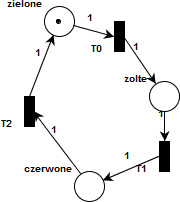
\includegraphics[width=4.5cm]{state_machine.png}\]

Stanami są miejsca sieci, zaś znacznik pokazuje w jakim stanie aktualnie
się znajdujemy.

\hypertarget{ux107wiczenia}{%
\subsubsection{Ćwiczenia:}\label{ux107wiczenia}}

\begin{itemize}
\tightlist
\item
  Narysować przykład w symulatorze
\item
  Sprawdzić właściwości sieci (ograniczoność, bezpieczenstwo i możliwy
  deadlock) w symulatorze Pipe w menu ``State Space Analysis''.
\item
  Wygenerować graf osiągalności ``Reachability/Coverability Graph''.
  Zaobserwować:

  \begin{itemize}
  \tightlist
  \item
    Jakie znakowania są osiągalne?
  \item
    Ile wynosi maksymalna liczba znaczników w każdym ze znakowań? Jakie
    możemy wyciągnac z tego wnioski n.t. ograniczoności i
    bezpieczenstwa?
  \item
    Czy kazde przejście jest przedstawione jako krawędź w grafie? Jaki z
    tego wniosek n.t. żywotności przejść?
  \item
    Czy wychodząc od dowolnego węzła grafu (znakowania) można wykonać
    dowolne przejście? Jaki z tego wniosek n.t. zywotnosci sieci? Czy sa
    możliwe zakleszczenia?
  \end{itemize}
\item
  Wykonać analizę niezmiennikow (wybrac w menu ``Invariant Analysis'').

  \begin{itemize}
  \tightlist
  \item
    Wynik analizy niezmienników przejść (T-invariants) pokazuje nam, ile
    razy trzeba odpalić dane przejście (T), aby przekształcić znakowanie
    początkowe z powrotem do niego samego (wynik nie mówi nic o
    kolejności odpaleń). Z wyniku mozemy m.in. wnioskować o
    odwracalności sieci.
  \item
    Wynik analizy niezmienników miejsc (P-invariants) pokazuje nam
    zbiory miejsc, w których łączna suma znaczników się nie zmienia.
    Pozwala to wnioskować n.t. zachowawczości sieci (czyli własności,
    gdzie suma znaczników pozostaje stała) oraz o ograniczoności miejsc.
  \end{itemize}
\end{itemize}

    \hypertarget{zadania}{%
\subsection{Zadania}\label{zadania}}

\begin{enumerate}
\def\labelenumi{\arabic{enumi}.}
\item
  Wymyślić własną maszynę stanów, zasymulować przykład i dokonać analizy
  grafu osiągalności oraz niezmienników j.w.
\item
  Zasymulować sieć jak poniżej:

  \begin{figure}
  \centering
  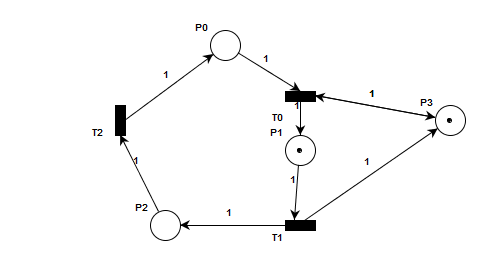
\includegraphics{task_2.png}
  \caption{task\_2.png}
  \end{figure}

  \begin{itemize}
  \tightlist
  \item
    Dokonać analizy niezmienników przejść. Jaki wniosek można wyciągnąć
    o odwracalności sieci?
  \item
    Wygenerować graf osiągalności. Proszę wywnioskować z grafu, czy sieć
    jest żywa.
  \item
    Proszę wywnioskować czy jest ograniczona. Objaśnić wniosek.
  \end{itemize}
\item
  Zasymulować wzajemne wykluczanie dwoch procesów na wspólnym zasobie.

  \begin{itemize}
  \tightlist
  \item
    Dokonać analizy niezmienników.
  \item
    Wyjaśnij znaczenie równań (P-invariant equations). Które równanie
    pokazuje działanie ochrony sekcji krytycznej?
  \end{itemize}
\item
  Uruchomić problem producenta i konsumenta z ograniczonym buforem
  (można posłużyć się przykładem, menu:file, examples).

  \begin{itemize}
  \tightlist
  \item
    Dokonać analizy niezmienników.
  \item
    Czy sieć jest zachowawcza?
  \item
    Ktore równanie mówi nam o rozmiarze bufora?
  \end{itemize}
\item
  Stworzyć symulacje problemu producenta i konsumenta z nieograniczonym
  buforem.

  \begin{itemize}
  \tightlist
  \item
    Dokonać analizy niezmienników.
  \item
    Zaobserwować brak pełnego pokrycia miejsc.
  \end{itemize}
\item
  Zasymulować prosty przykład ilustrujący zakleszczenie.

  \begin{itemize}
  \tightlist
  \item
    Wygenerować graf osiągalności i zaobserwować znakowania, z których
    nie można wykonać przejść.
  \item
    Zaobserwować właściwości sieci w ``State Space Analysis''.
  \end{itemize}

  Poniżej przykład sieci z możliwością zakleszczenia (można wymyślić
  inny):

  \begin{figure}
  \centering
  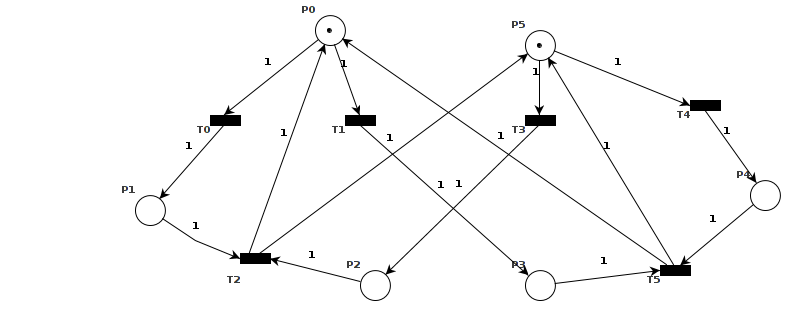
\includegraphics{task_6.png}
  \caption{task\_6.png}
  \end{figure}
\end{enumerate}

    \hypertarget{wstux119p-teoretyczny}{%
\section{Wstęp teoretyczny}\label{wstux119p-teoretyczny}}

\begin{itemize}
\item
  \textbf{Sieci Petriego} - narzędzie wprowadzone przez Carla A.
  Petriego w 1962 roku do pierwotnie modelowania komunikacji z
  automatami. Obecnie narzędzie stosowane jest w modelowaniu systemów
  współbieżnych, dyskretnych, synchronizacji procesów i wielu innych.
\item
  Własności:

  \begin{itemize}
  \tightlist
  \item
    \textbf{Ograniczoność}: odnosi się do maksymalnej liczby żetonów,
    które mogą znajdować się w danym miejscu. Sieć Petriego jest
    ograniczona, jeśli w żadnym z jej miejsc w trakcie działania sieci
    liczba żetonów (znaczników) nie może rosnąć w nieskończoność. Innymi
    słowy, istnieje pewna maksymalna liczba żetonów, która może
    znajdować się w każdym miejscu w dowolnym momencie.
  \item
    \textbf{Bezpieczeństwo}: to specjalny przypadek ograniczoności,
    gdzie maksymalna liczba żetonów w miejscu wynosi 1.
  \item
    \textbf{Deadlock}: stan, w którym żadne dalsze przejścia nie są
    możliwe.
  \item
    \textbf{Zachowawczość sieci}: własność, gdzie suma żetonów pozostaje
    stała.
  \item
    \textbf{Żywotność sieci} -- każde przejście ma szanse się wykonać.
  \item
    \textbf{Żywotność miejsca} -- miejsce ma szanse zawierać znaczniki.
  \item
    \textbf{Żywotność przejścia} -- przejście ma szanse się wykonać.
  \item
    \textbf{Odwracalność} oznacza, że istnieje możliwość powrotu do
    stanu początkowego (początkowego znakowania) z dowolnego innego
    stanu (znakowania) sieci. Innymi słowy, jeśli sieć jest odwracalna,
    to znaczy, że po serii przejść (odpalenia tranzycji) można wrócić do
    stanu początkowego.
  \end{itemize}
\item
  \textbf{Graf osiągalności} obrazuje zmienianie się warunków logicznych
  (lokalnych stanów).
\item
  \textbf{Znaczniki} to żetony (tokeny), które można przemieszczać
  pomiędzy miejscami poprzez przejścia, po krawędziach grafu.
\item
  Znaczniki (tokeny, żetony) prezentowane są graficznie w postaci kropek
  umieszczanych w kółkach reprezentujących miejsca.
\item
  \textbf{Niezmienniki przejść (T-invariants)} pokazują, ile razy trzeba
  odpalić dane przejście (T), aby przekształcić znakowanie początkowe z
  powrotem do niego samego.
\item
  \textbf{Niezmienniki miejsc (P-invariants)} pokazują zbiory miejsc, w
  których łączna suma znaczników się nie zmienia. Pozwala to wnioskować
  o zachowawczości sieci oraz o ograniczoności miejsc.
\item
  \textbf{Równania (P-invariant equations)} są związane z niezmiennikami
  miejsc i pokazują zbiory miejsc, w których łączna suma znaczników się
  nie zmienia.
\end{itemize}

    \hypertarget{rozwiux105zania}{%
\section{Rozwiązania}\label{rozwiux105zania}}

    \hypertarget{maszyna-stanuxf3w}{%
\subsection{Maszyna stanów}\label{maszyna-stanuxf3w}}

    Maszyna została narysowana w symulatorze w sposób następujący:

\begin{figure}
\centering
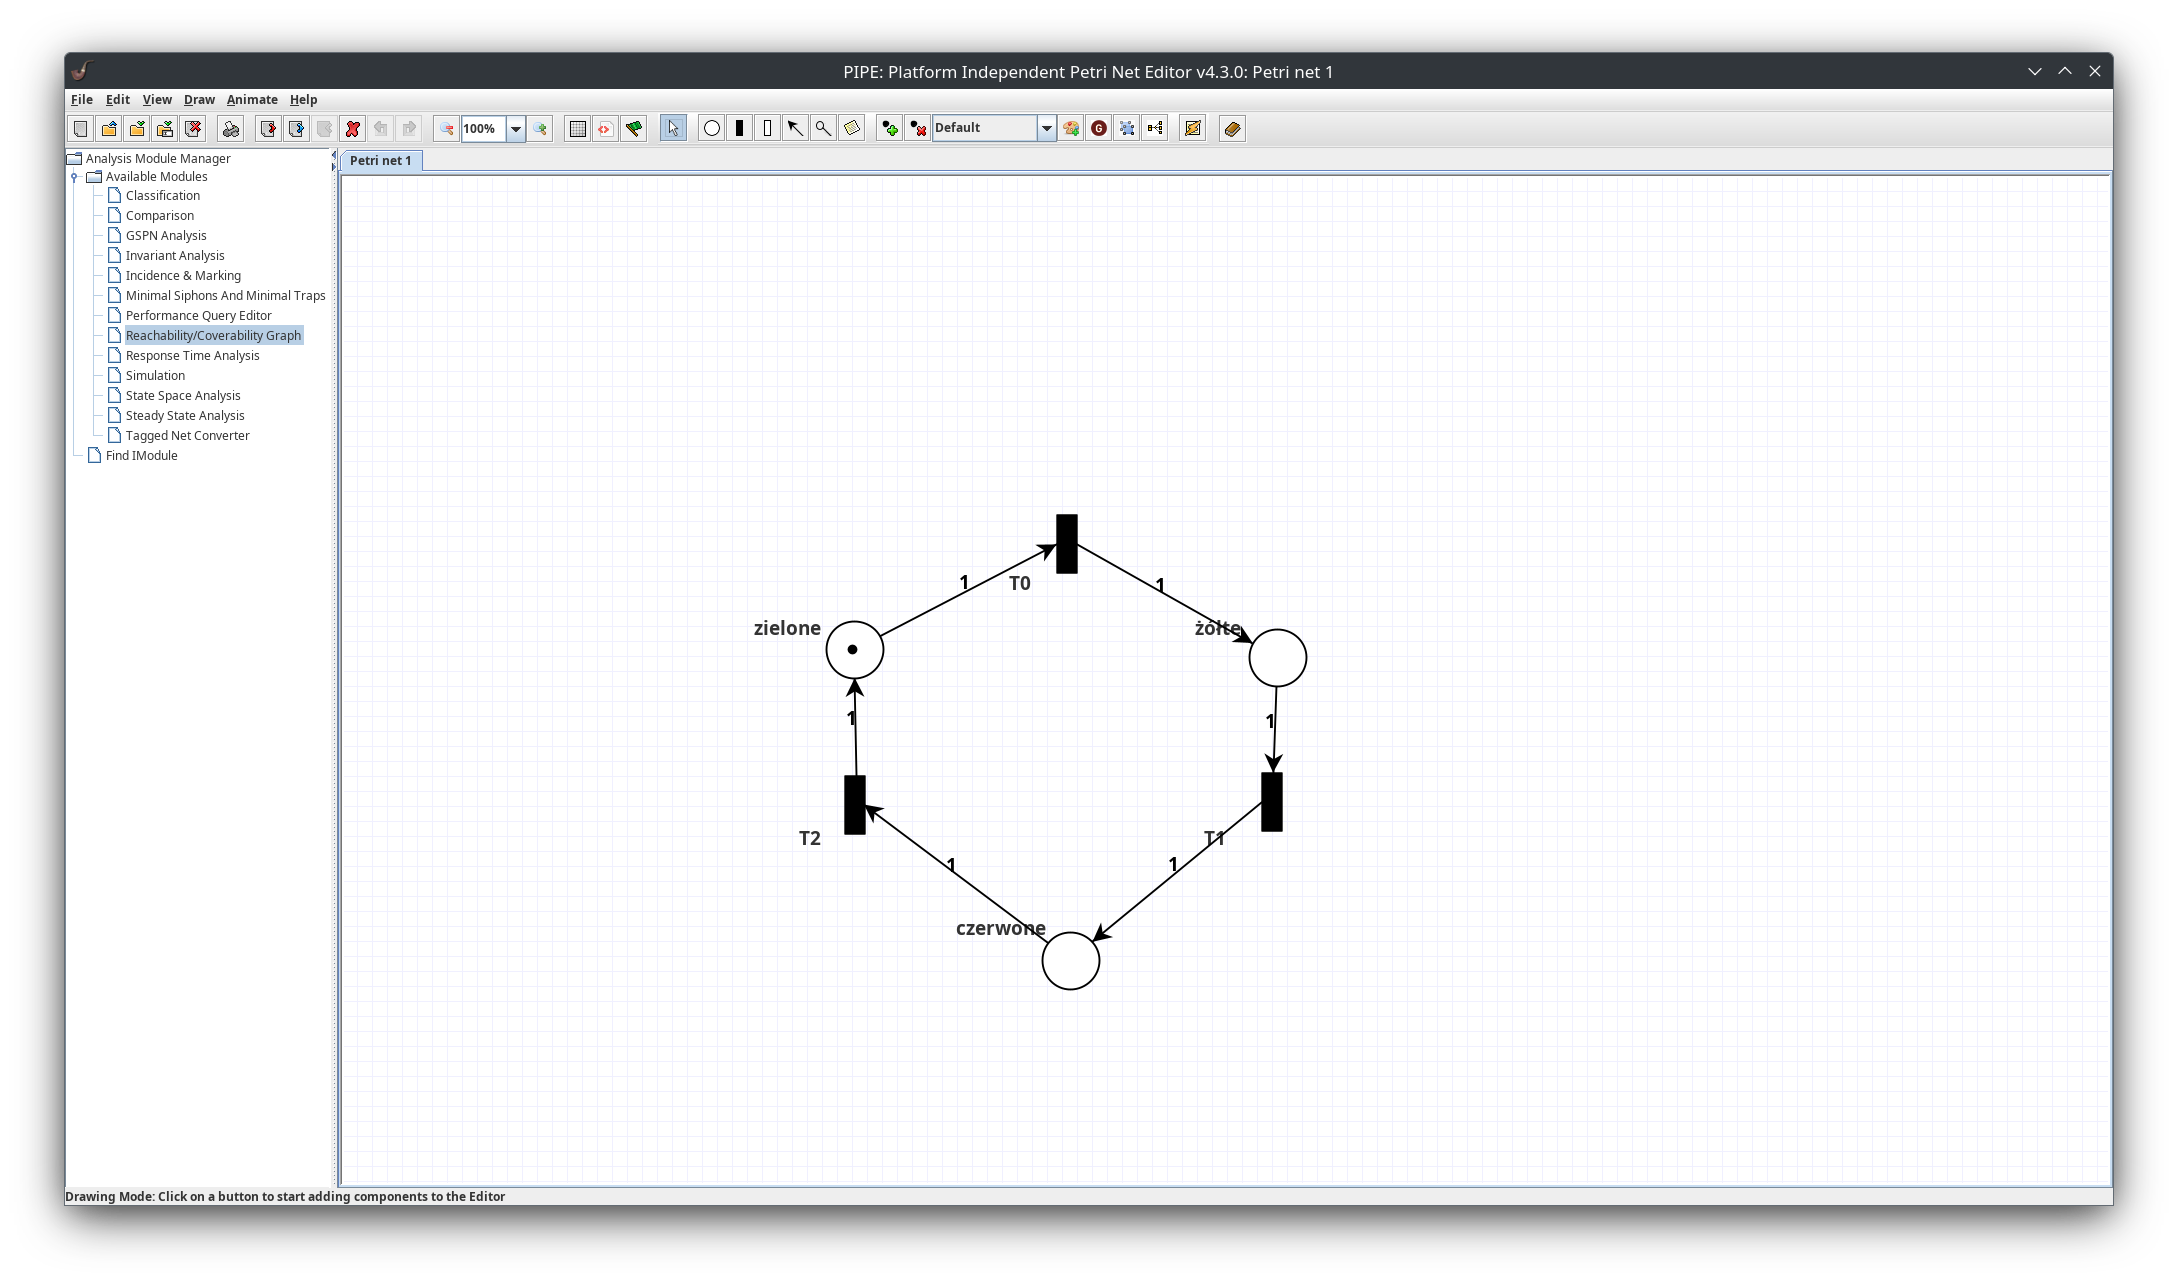
\includegraphics{Screenshot_20240106_205152.png}
\caption{Screenshot\_20240106\_205152.png}
\end{figure}

\hypertarget{analiza-stanuxf3w}{%
\subsubsection{Analiza stanów}\label{analiza-stanuxf3w}}

Jak wynika z \emph{State Space Analysis}, ta sieć jest:

\begin{itemize}
\tightlist
\item
  Ograniczona
\item
  Bezpieczna
\item
  Nie zawiera deadlocku
\end{itemize}

\[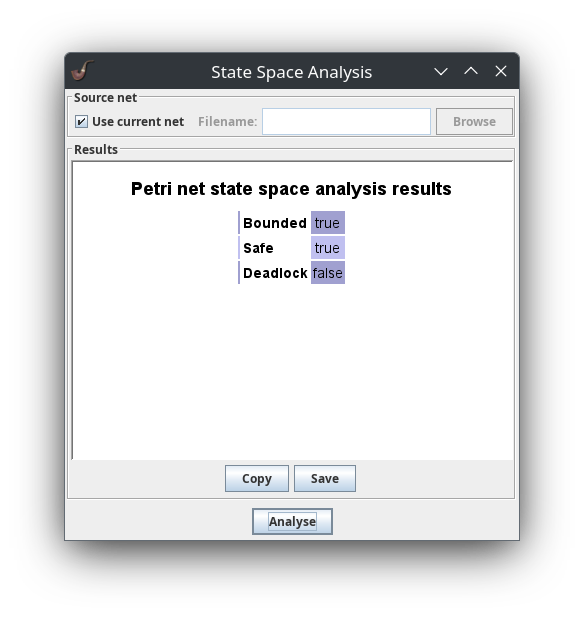
\includegraphics[width=7cm]{Screenshot_20240106_205310.png}\]

    \hypertarget{graf-osiux105galnoux15bci}{%
\subsubsection{Graf osiągalności}\label{graf-osiux105galnoux15bci}}

Graf osiągalności został wygenerowany i wygląda w sposób następujący:

\begin{figure}
\centering
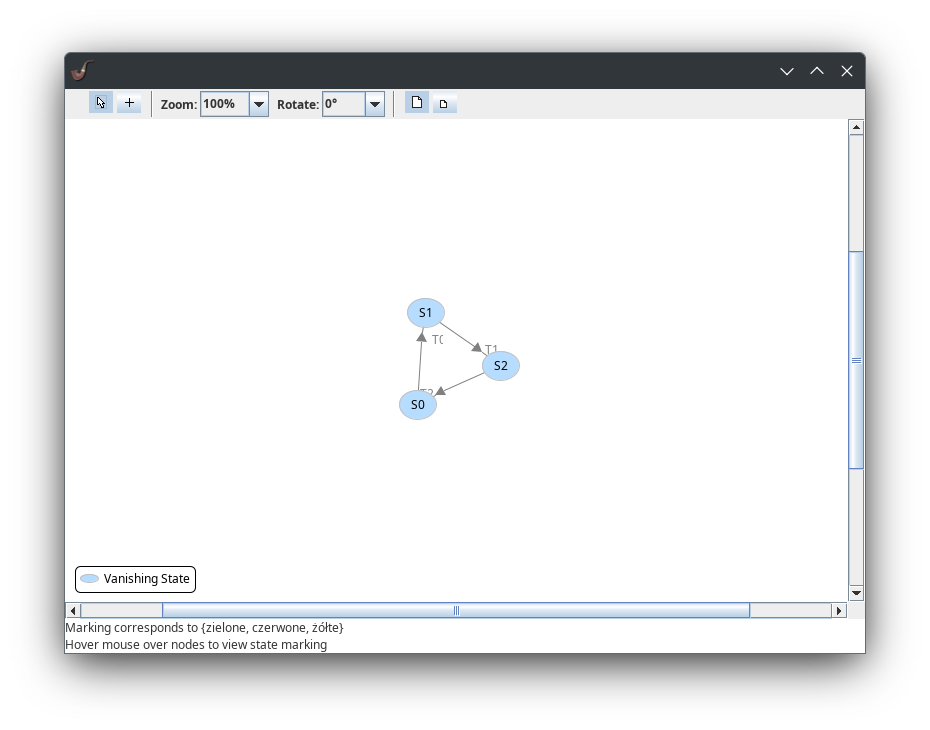
\includegraphics{Screenshot_20240106_205607.png}
\caption{Screenshot\_20240106\_205607.png}
\end{figure}

\begin{itemize}
\item
  Jak widać z powyższego grafu, \textbf{wszystkie znakowania} (stany,
  \(S_0\), \(S_1\), \(S_2\)) \textbf{są osiągalne}.
\item
  W każdym ze znakowań maksymalna liczba znaczników (tokenów) wynosi 1.
  Cała ta maszyna stanów zawiera tylko 1 token, reprezentujący obecny
  stan. Przejście między poszczególnymi stanami odbywa się sekwencyjnie.
  A więc dana sieć jest \textbf{ograniczona} i \textbf{bezpieczna}.
\item
  Każde przejście (\(T_0\), \(T_1\), \(T_2\)) jest przedstawione jako
  osobna krawędź w grafie. To świadczy o tym, że każde przejście ma
  szansę się wykonać - a więc \textbf{wszystkie przejścia są żywe}.
\item
  Tak, wychodząc od dowolnego węzła grafu w \(k\) krokach można wykonać
  dowolne przejście. To świadczy o tym, że \textbf{sieć jest żywa} -
  każde przejście ma szansę się wykonać.
\end{itemize}

    \hypertarget{analiza-niezmiennikuxf3w}{%
\subsubsection{Analiza niezmienników}\label{analiza-niezmiennikuxf3w}}

Wynik dokonanej analizy niezmienników jest widoczny na obrazku poniżej:

\[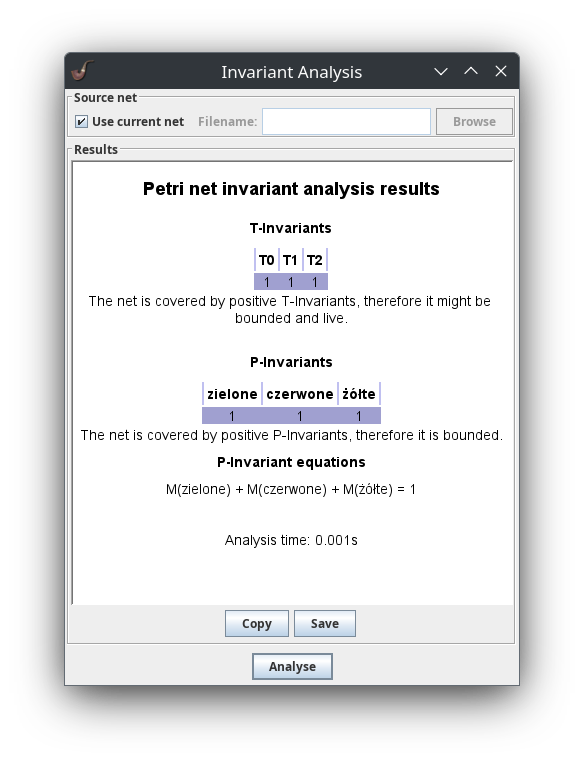
\includegraphics[width=7cm]{Screenshot_20240106_212923.png}\]

    \hypertarget{zadanie-1}{%
\subsection{Zadanie 1}\label{zadanie-1}}

Sieć, reprezentująca równoległe wykonanie czynności:

\begin{figure}
\centering
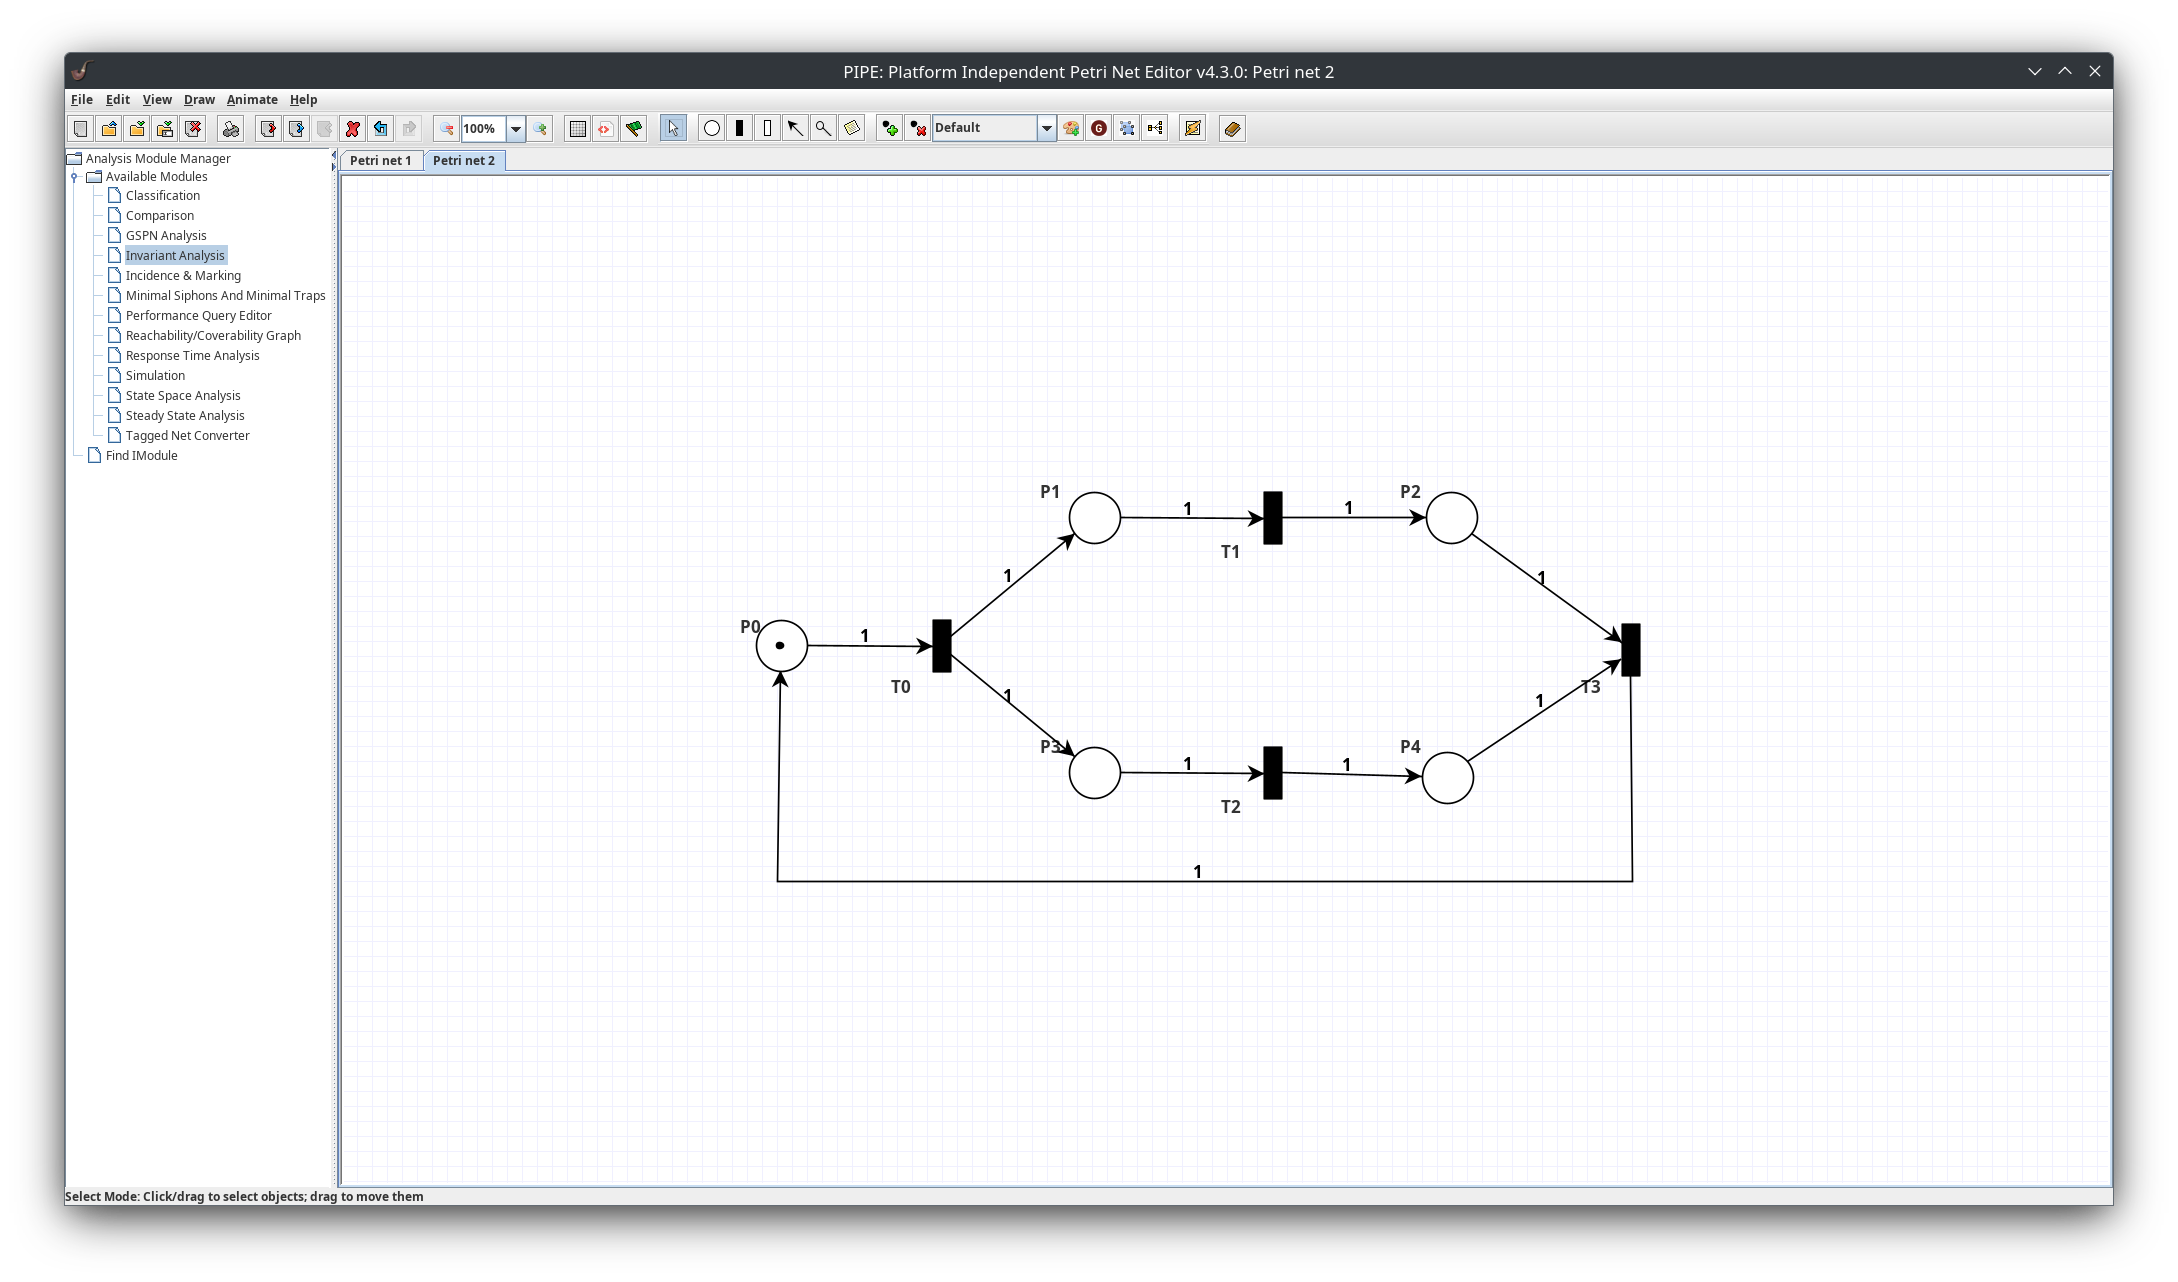
\includegraphics{Screenshot_20240106_215810.png}
\caption{Screenshot\_20240106\_215810.png}
\end{figure}

    \hypertarget{analiza-stanuxf3w}{%
\subsubsection{Analiza stanów}\label{analiza-stanuxf3w}}

Jak wynika z \emph{State Space Analysis}, ta sieć jest:

\begin{itemize}
\tightlist
\item
  Ograniczona
\item
  Bezpieczna
\item
  Nie zawiera deadlocku
\end{itemize}

\[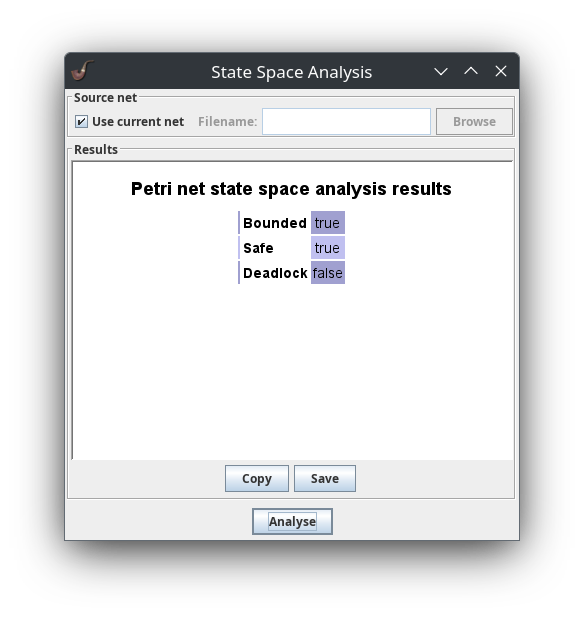
\includegraphics[width=7cm]{Screenshot_20240107_135913.png}\]

    \hypertarget{graf-osiux105galnoux15bci}{%
\subsubsection{Graf osiągalności}\label{graf-osiux105galnoux15bci}}

Graf osiągalności został wygenerowany i wygląda w sposób następujący:

\begin{figure}
\centering
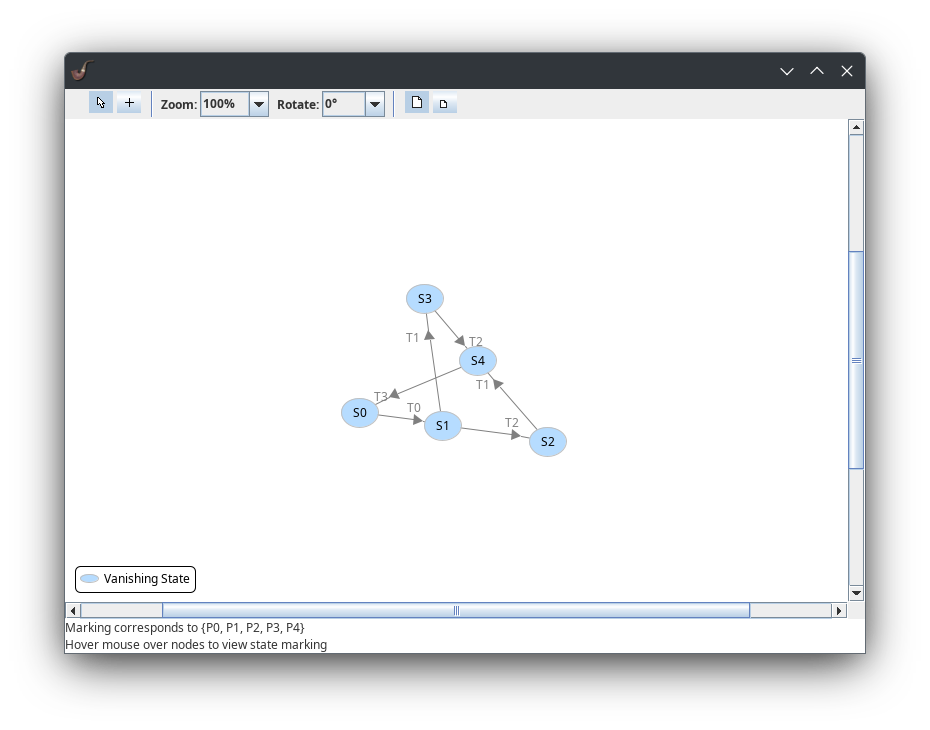
\includegraphics{Screenshot_20240107_140252.png}
\caption{Screenshot\_20240107\_140252.png}
\end{figure}

W odróżnieniu od poprzedniego przypadku, w tym przypadku jeden stan
(\(S_i\)) może reprezentować kilka miejsc (\(P_j\)) naraz (bo
``zadania'' wykonują się równolegle):

\begin{itemize}
\tightlist
\item
  \(S_0 = \{P_0\}\)
\item
  \(S_1 = \{P_1, P_3\}\)
\item
  \(S_2 = \{P_1, P_4\}\)
\item
  \(S_3 = \{P_2, P_3\}\)
\item
  \(S_4 = \{P_2, P_4\}\)
\end{itemize}

Ponadto:

\begin{itemize}
\tightlist
\item
  Jak widać z powyższego grafu, \textbf{wszystkie znakowania są
  osiągalne}.
\item
  W każdym ze znakowań maksymalna liczba znaczników (tokenów) wynosi 1.
  Z tego wynika, że ta \textbf{sieć jest ograniczona i bezpieczna}.
\item
  Każde przejście (\(T_0\), \(T_1\), \(T_2\), \(T_3\)) jest
  przedstawione jako osobna krawędź (osobne krawędzie) w grafie. To
  świadczy o tym, że każde przejście ma szansę się wykonać - a więc
  \textbf{wszystkie przejścia są żywe}.
\item
  Tak, wychodząc od dowolnego węzła grafu w \(k\) krokach można wykonać
  dowolne przejście. To świadczy o tym, że \textbf{sieć jest żywa} -
  każde przejście ma szansę się wykonać.
\end{itemize}

    \hypertarget{analiza-niezmiennikuxf3w}{%
\subsubsection{Analiza niezmienników}\label{analiza-niezmiennikuxf3w}}

Wynik dokonanej analizy niezmienników jest przedstawiony na obrazku
poniżej:

\[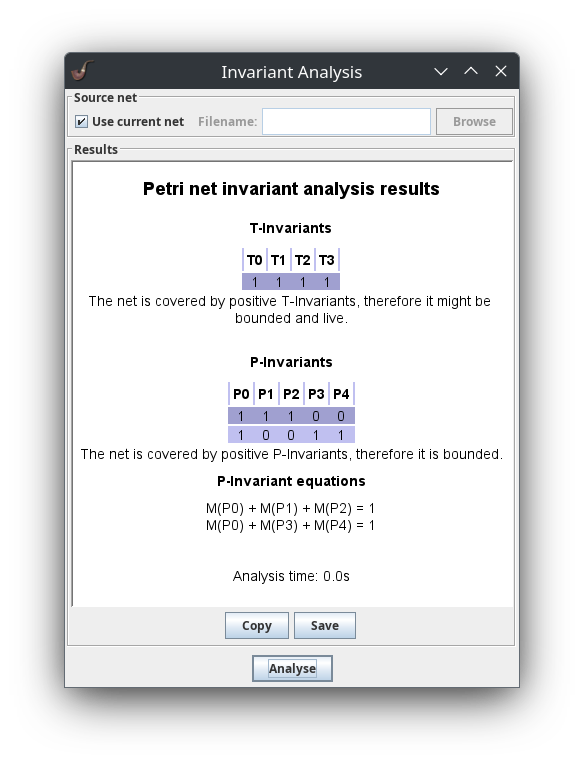
\includegraphics[width=7cm]{Screenshot_20240107_141544.png}\]

    \hypertarget{zadanie-2}{%
\subsection{Zadanie 2}\label{zadanie-2}}

Sieć została narysowana w symulatorze w sposób następujący:

\begin{figure}
\centering
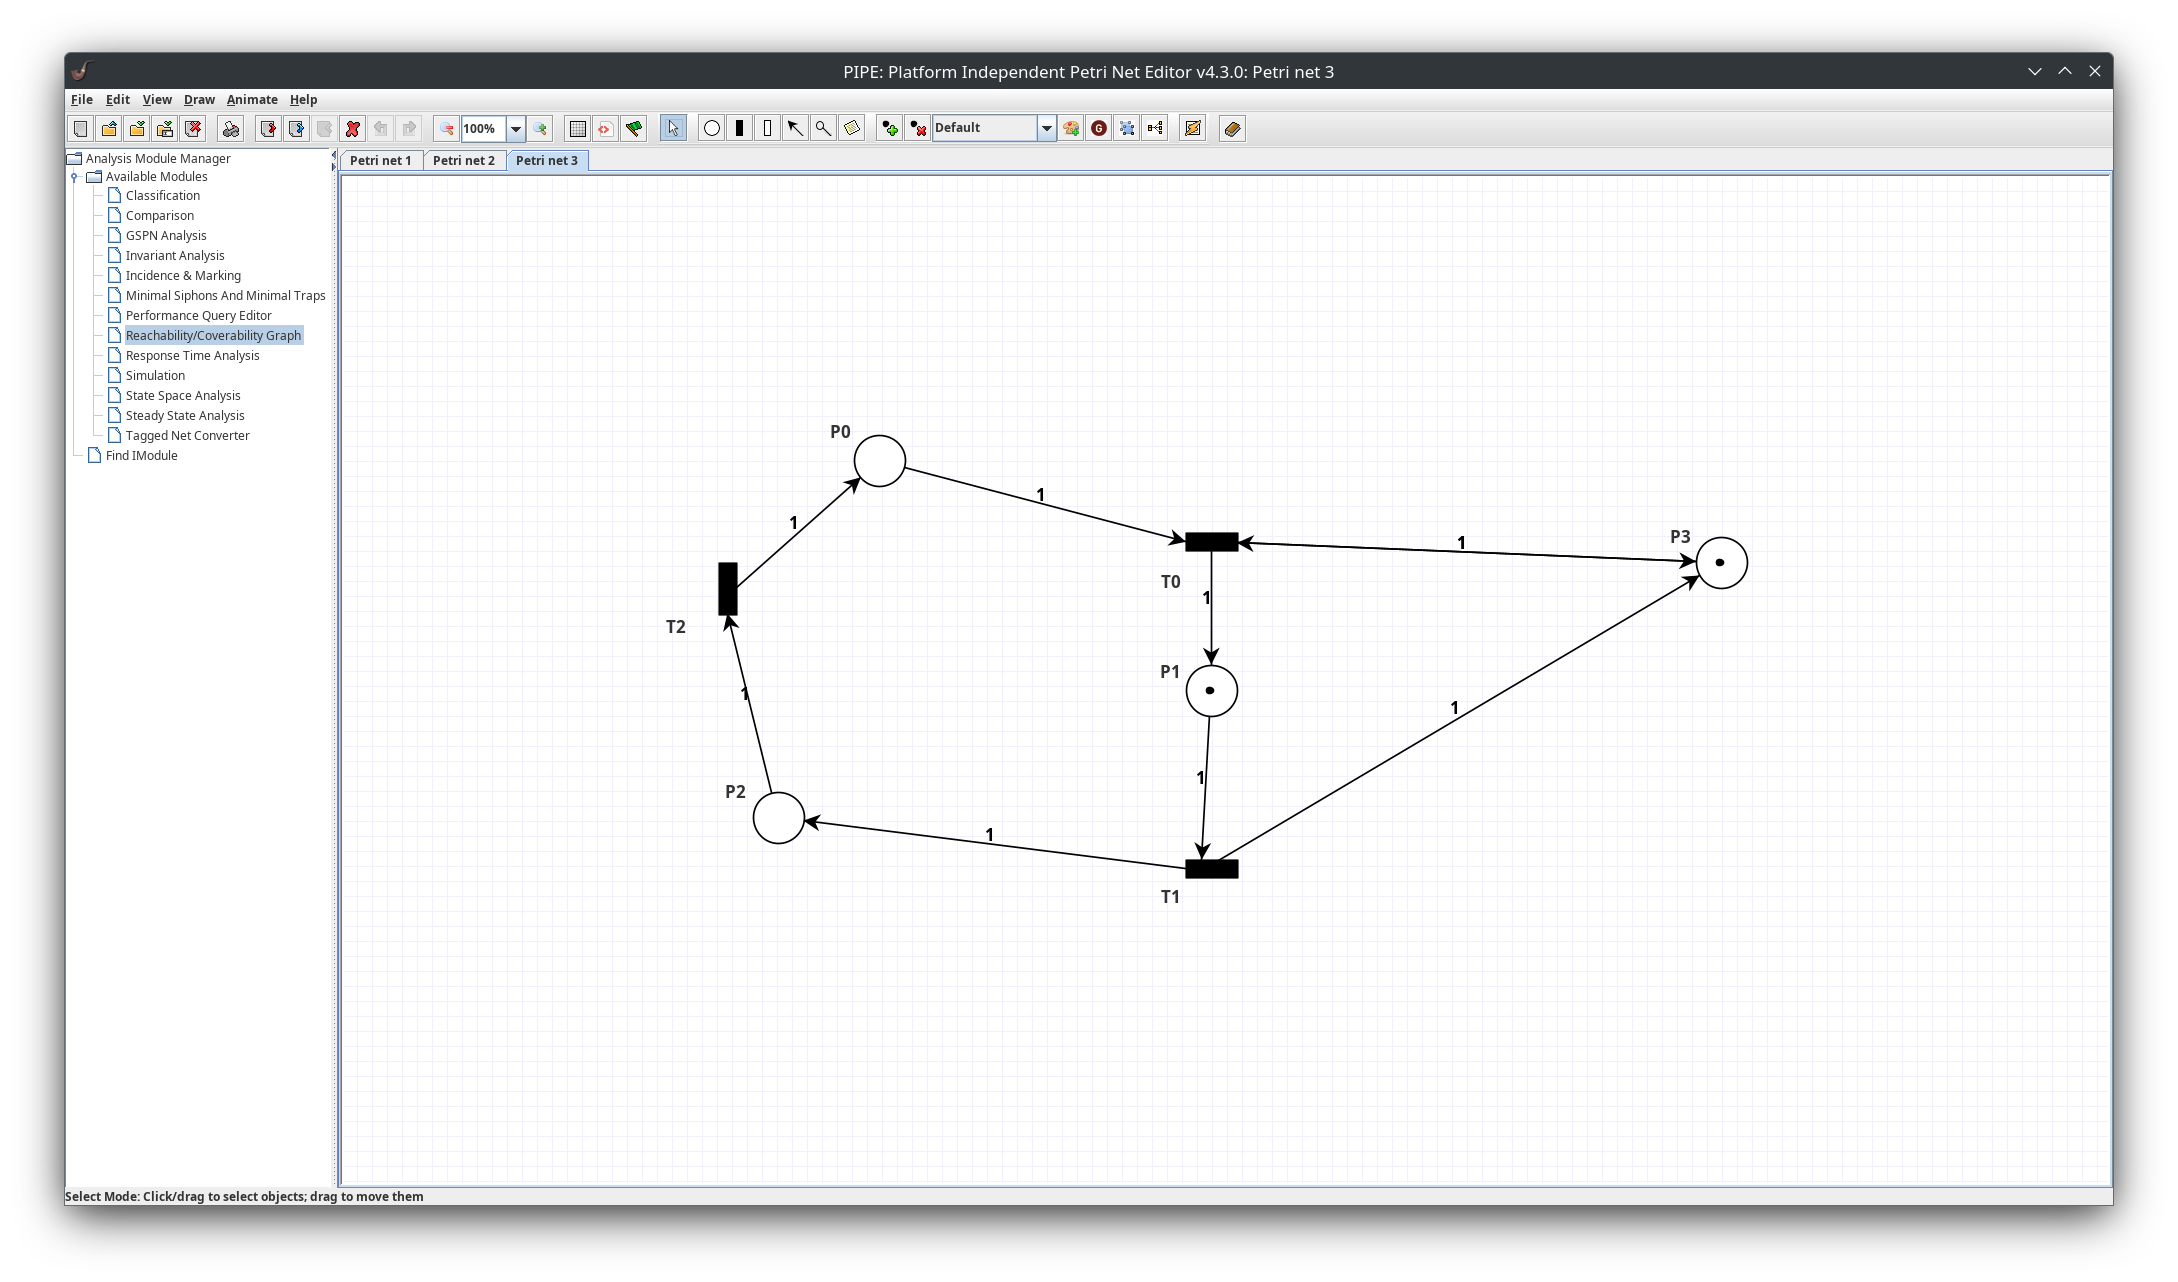
\includegraphics{Screenshot_20240107_142713.png}
\caption{Screenshot\_20240107\_142713.png}
\end{figure}

    \hypertarget{analiza-niezmiennikuxf3w}{%
\subsubsection{Analiza niezmienników}\label{analiza-niezmiennikuxf3w}}

Wynik dokonanej analizy niezmienników jest przedstawiony na obrazku
poniżej:

\[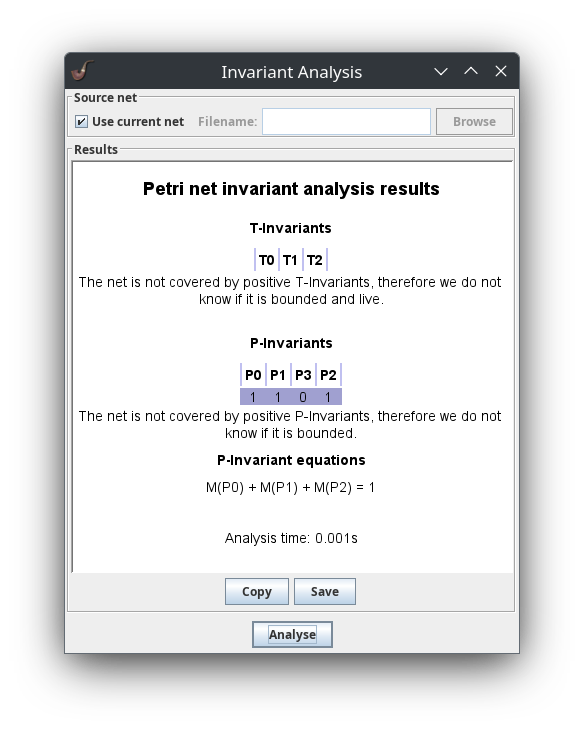
\includegraphics[width=7cm]{Screenshot_20240107_142750.png}\]

Na podstawie otrzymanych informacji nie można wyciągnąć żadnych wniosków
co do tej sieci.

    \hypertarget{analiza-stanuxf3w}{%
\subsubsection{Analiza stanów}\label{analiza-stanuxf3w}}

Z kolei analiza stanów pozwala stwierdzić, że sieć:

\begin{itemize}
\tightlist
\item
  Nie jest ograniczona
\item
  Nie jest bezpieczna
\item
  Nie zawiera deadlocku
\end{itemize}

\[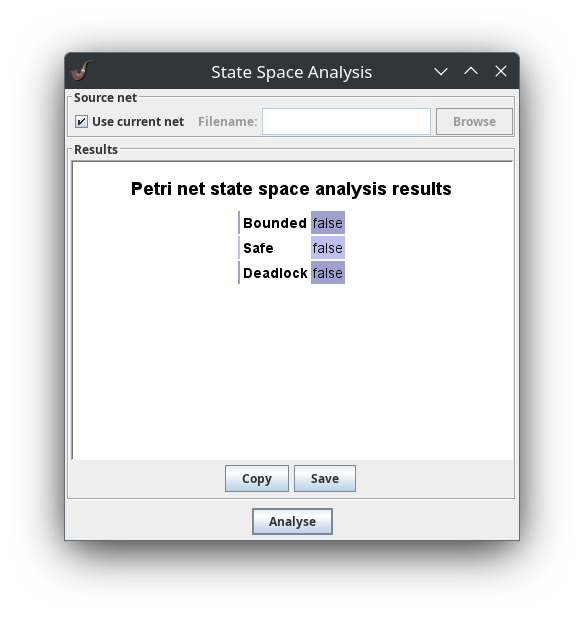
\includegraphics[width=7cm]{Screenshot_20240107_142908.png}\]

    \hypertarget{graf-osiux105galnoux15bci}{%
\subsubsection{Graf osiągalności}\label{graf-osiux105galnoux15bci}}

Został wygenerowany następujący graf osiągalności:

\begin{figure}
\centering
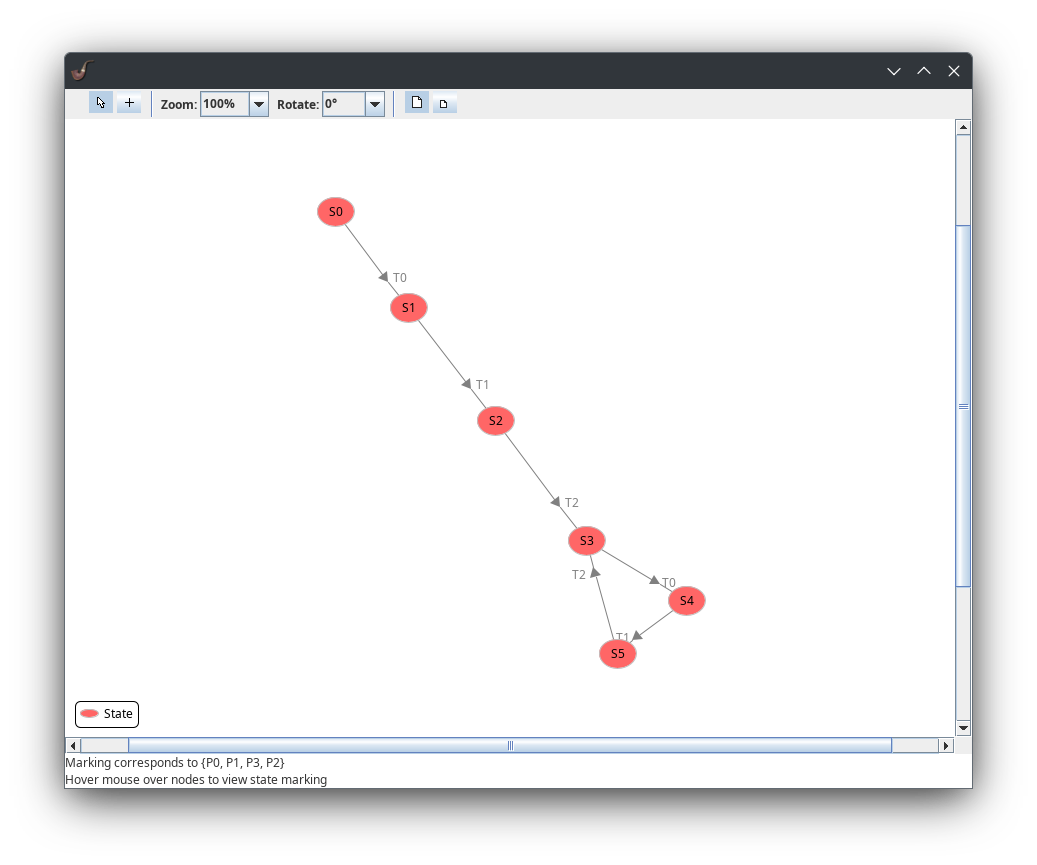
\includegraphics{Screenshot_20240107_143257.png}
\caption{Screenshot\_20240107\_143257.png}
\end{figure}

Co ciekawe, wygenerowanie tego grafu zajęło ponad 17 sekund.

\textbf{Sieć jest żywa} - wychodząc od dowolnego węzła grafu w \(k\)
krokach można wykonać dowolne przejście (\(T_0\), \(T_1\), \(T_2\)). A
więc każde przejście ma szansę się wykonać.

    \hypertarget{zadanie-3}{%
\subsection{Zadanie 3}\label{zadanie-3}}

Sieć symulująca wykluczanie dwoch procesów na wspólnym zasobie wygląda w
sposób następujący:

\begin{figure}
\centering
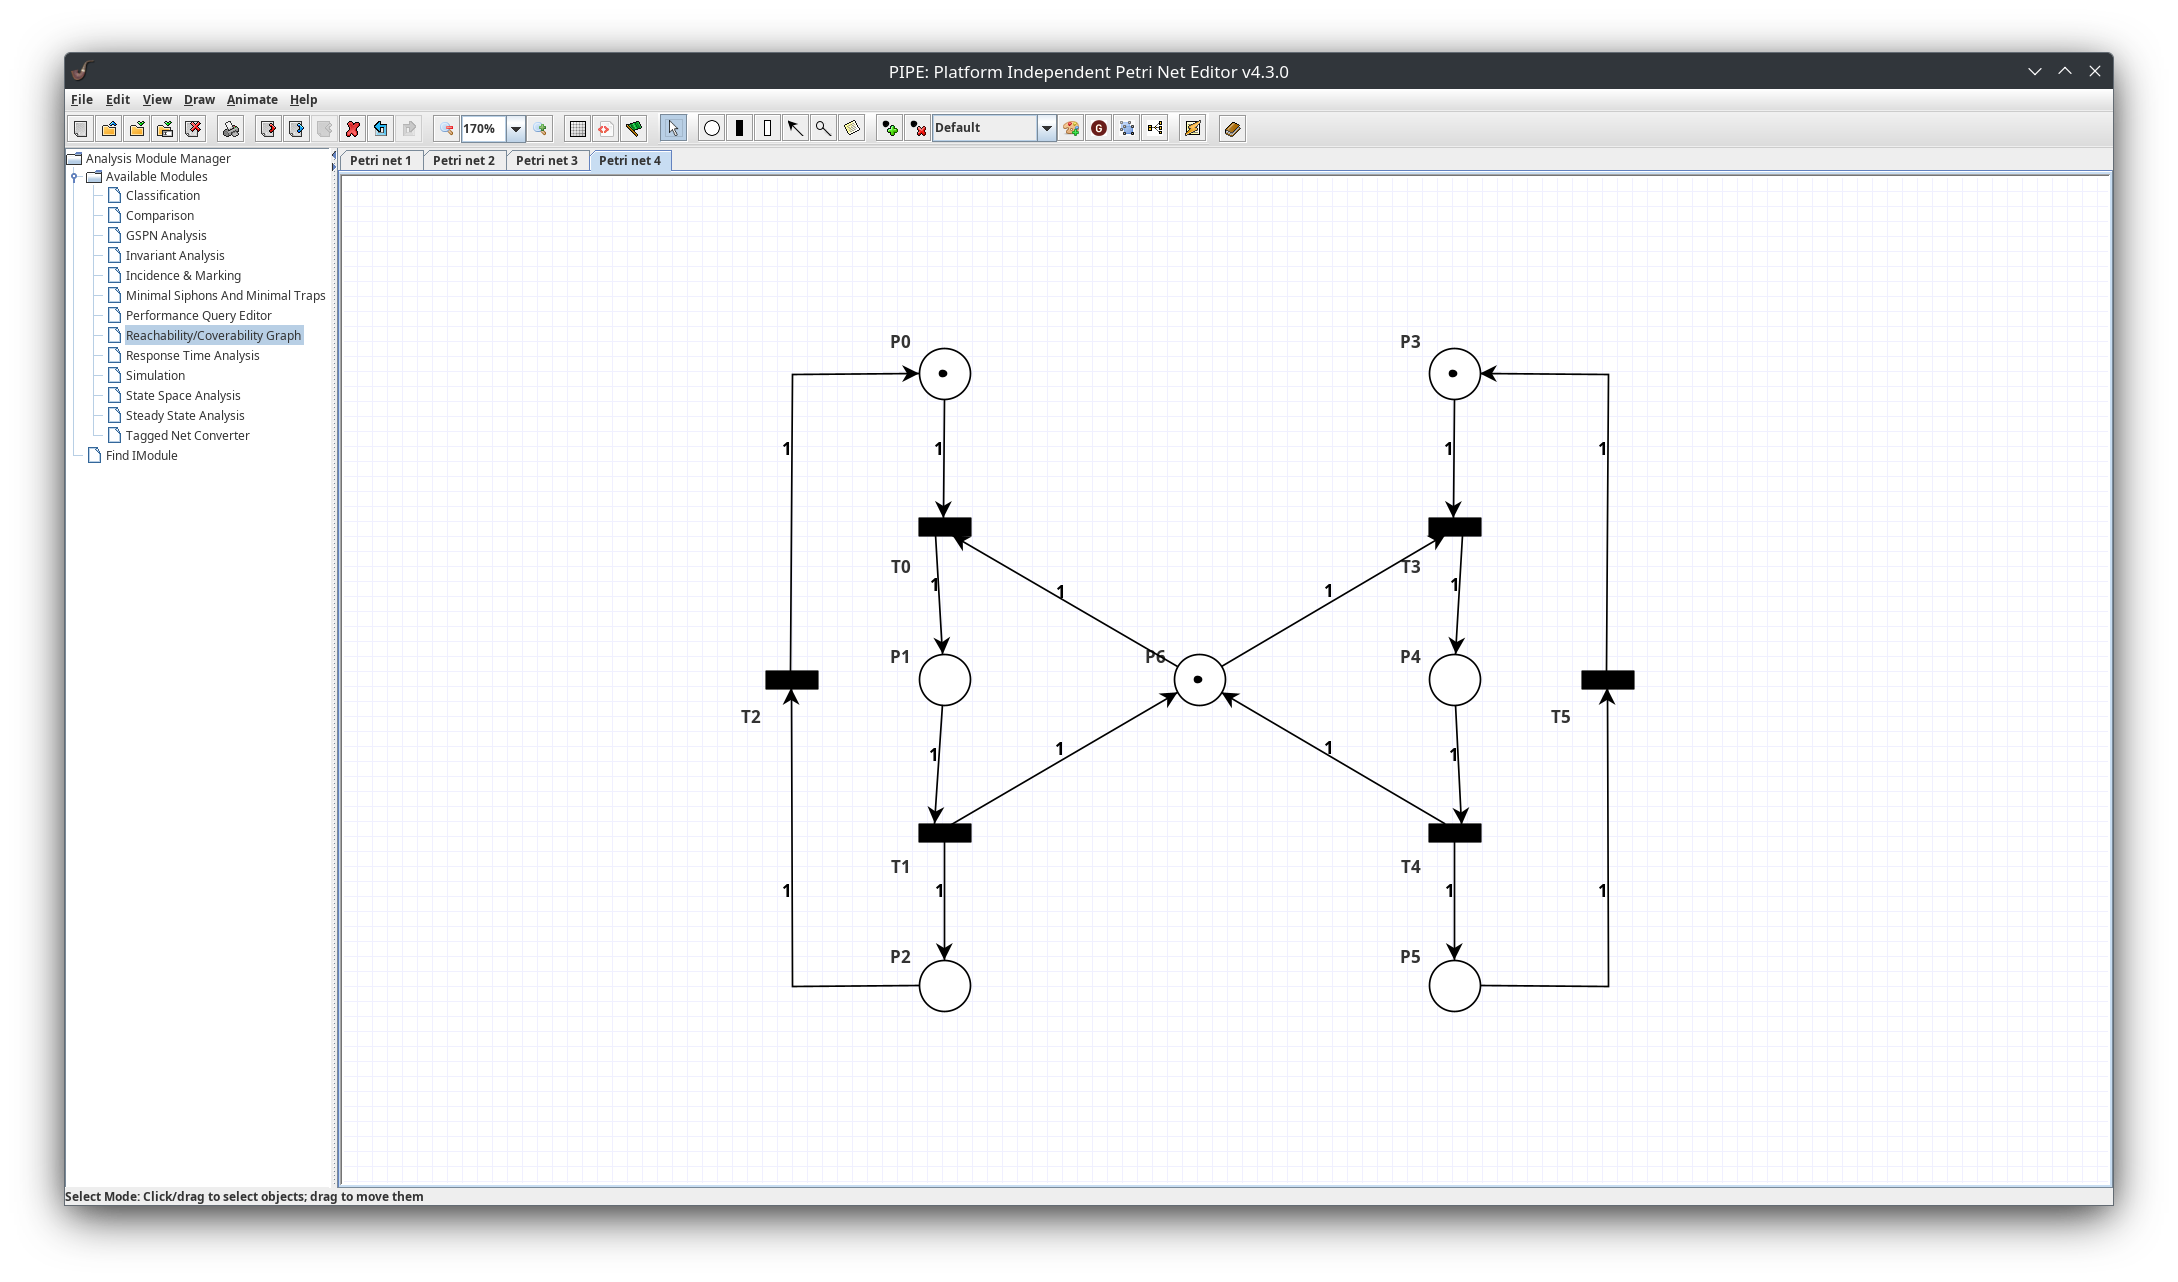
\includegraphics{Screenshot_20240107_144710.png}
\caption{Screenshot\_20240107\_144710.png}
\end{figure}

    \hypertarget{analiza-niezmiennikuxf3w}{%
\subsubsection{Analiza niezmienników}\label{analiza-niezmiennikuxf3w}}

Wynik dokonanej analizy niezmienników jest przedstawiony na obrazku
poniżej:

\[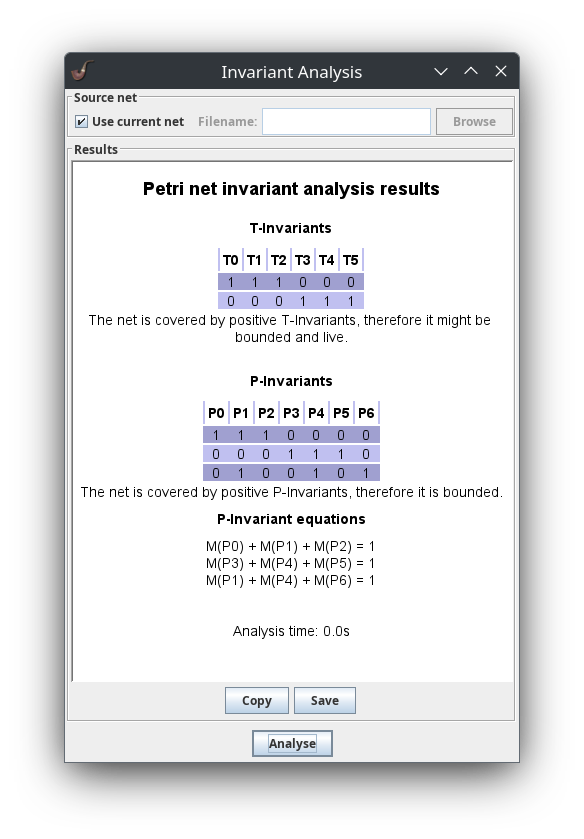
\includegraphics[width=7cm]{Screenshot_20240107_144801.png}\]

Ostatnie równanie, czyli \(M(P_1) + M(P_4) + M(P_6) = 1\) pokazuje
działanie ochrony sekcji krytycznej.

    \hypertarget{analiza-stanuxf3w}{%
\subsubsection{Analiza stanów}\label{analiza-stanuxf3w}}

Jak wynika z \emph{State Space Analysis}, ta sieć jest:

\begin{itemize}
\tightlist
\item
  Ograniczona
\item
  Bezpieczna
\item
  Nie zawiera deadlocku
\end{itemize}

\[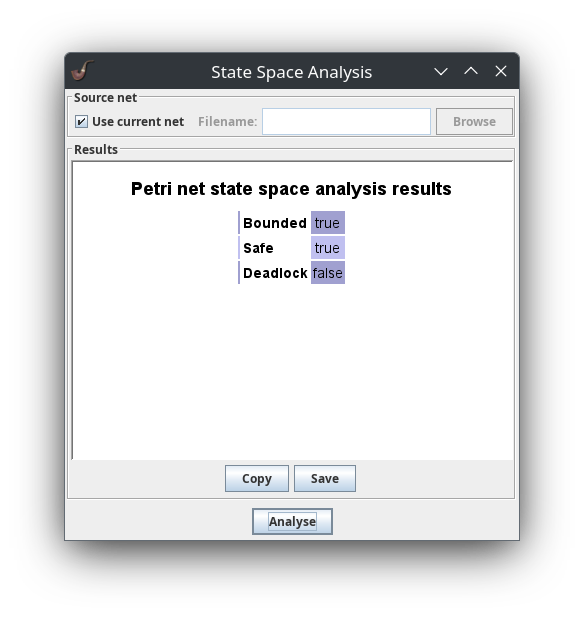
\includegraphics[width=7cm]{Screenshot_20240107_144927.png}\]

    \hypertarget{zadanie-4}{%
\subsection{Zadanie 4}\label{zadanie-4}}

Sieć reprezentująca problem producenta i konsumenta z ograniczonym
buforem wygląda następująco:

\begin{figure}
\centering
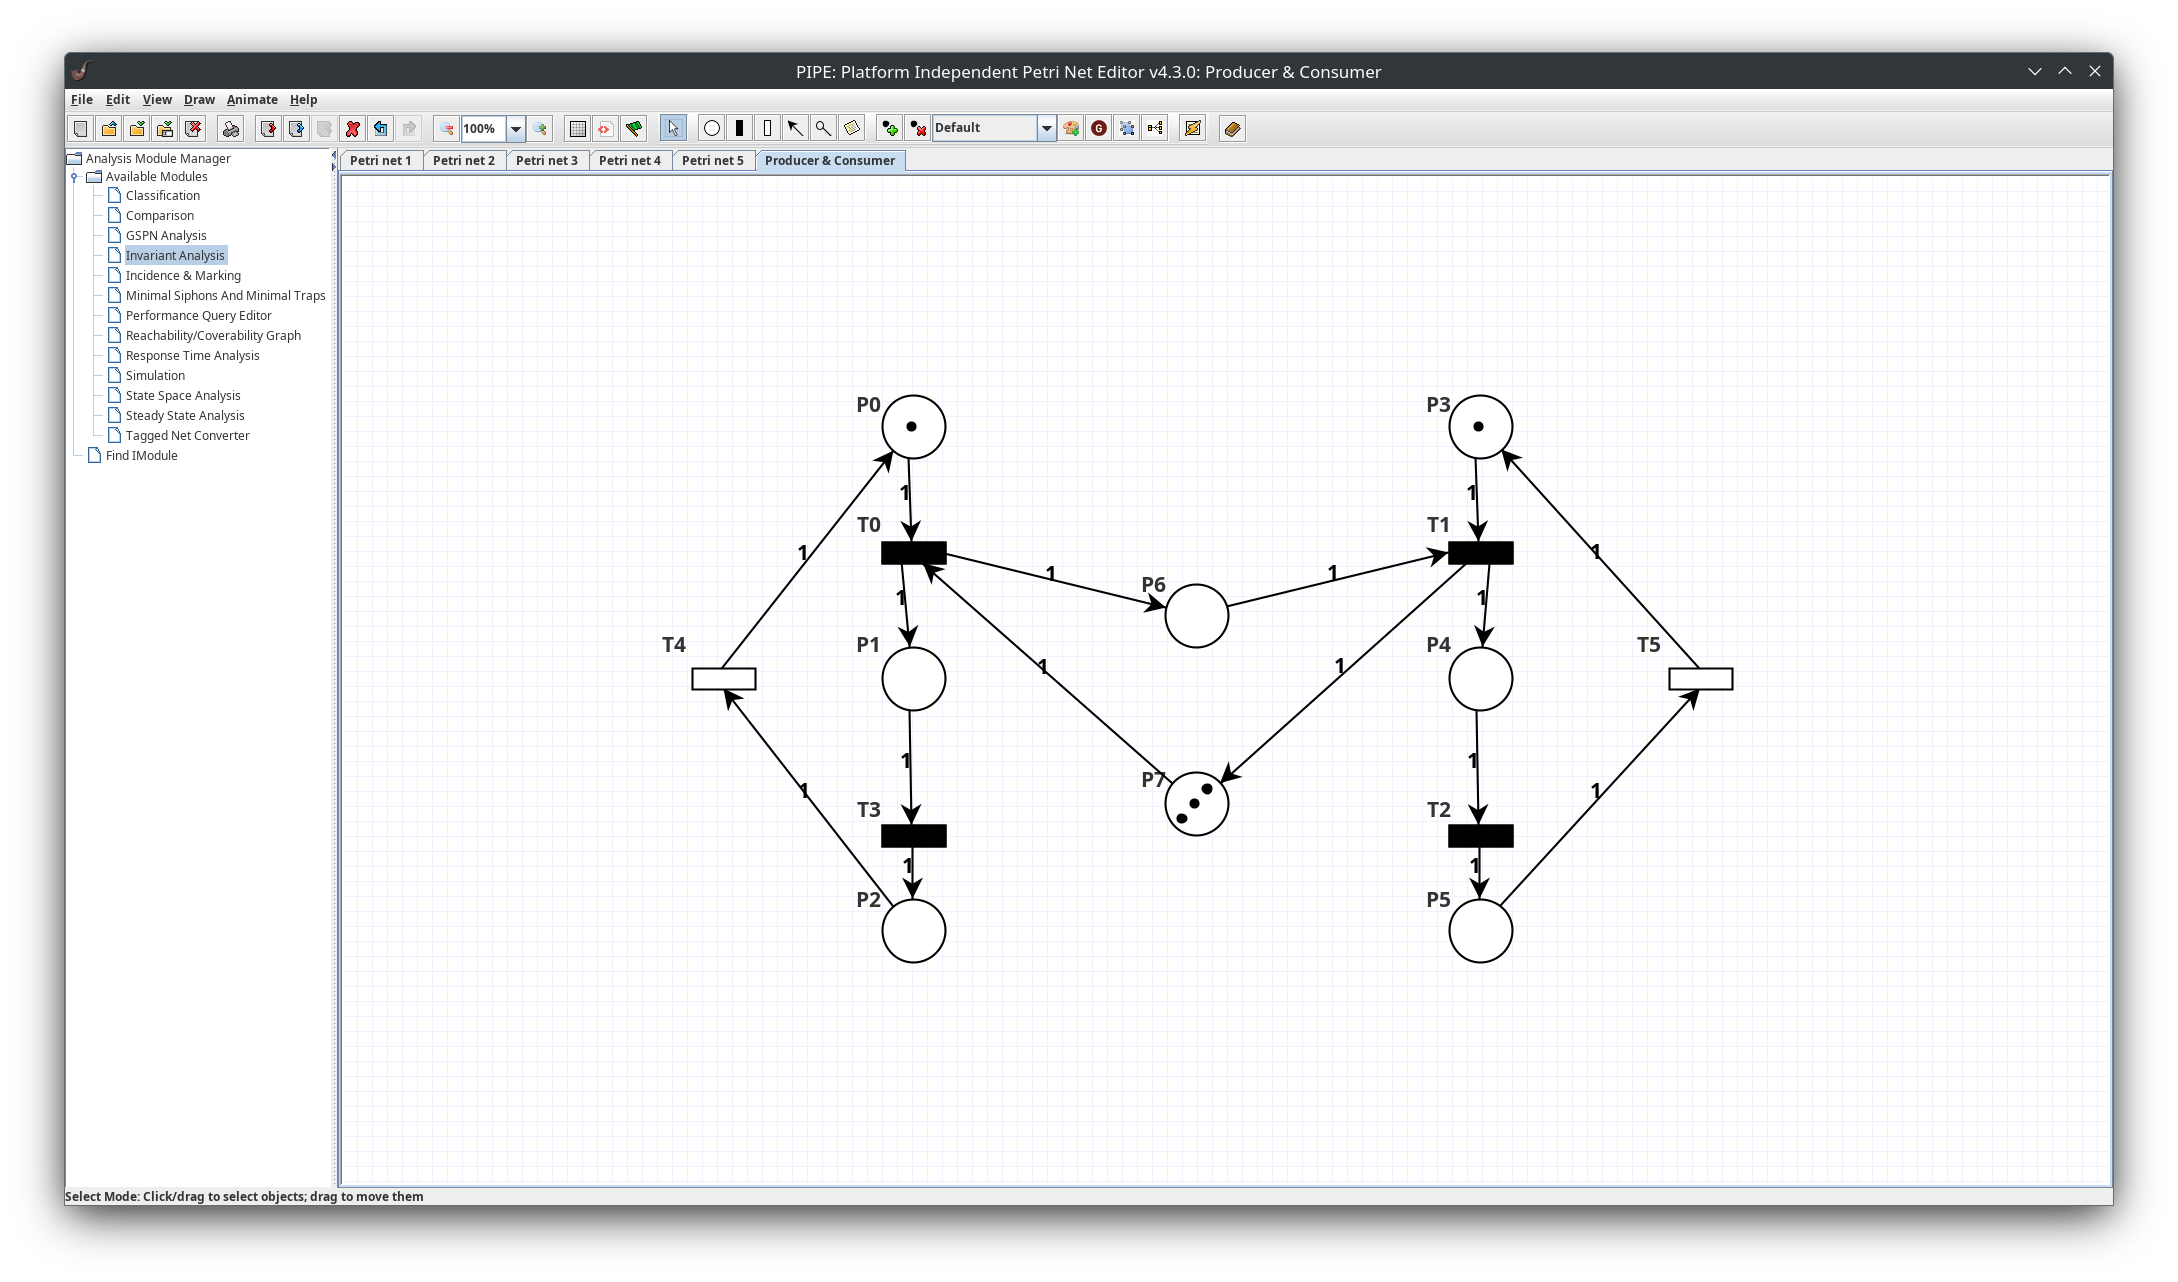
\includegraphics{Screenshot_20240107_145542.png}
\caption{Screenshot\_20240107\_145542.png}
\end{figure}

    \hypertarget{analiza-niezmiennikuxf3w}{%
\subsubsection{Analiza niezmienników}\label{analiza-niezmiennikuxf3w}}

Wynik dokonanej analizy niezmienników jest przedstawiony na obrazku
poniżej:

\[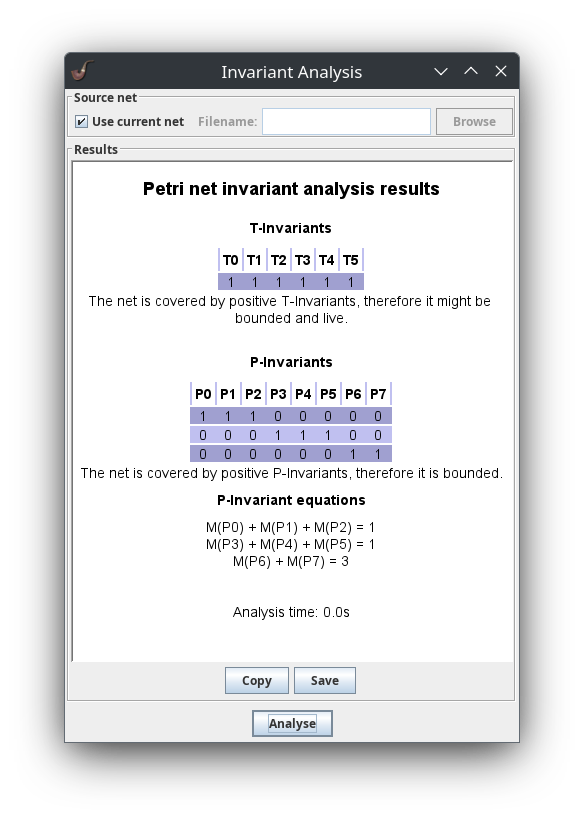
\includegraphics[width=7cm]{Screenshot_20240107_150005.png}\]

Ostatnie równanie, czyli \(M(P_6) + M(P_7) = 3\) mówi nam o rozmiarze
bufora.

\textbf{Sieć jest zachowawcza} - suma żetonów (tokenów, znaczników)
pozostaje stała.

    \hypertarget{analiza-stanuxf3w}{%
\subsubsection{Analiza stanów}\label{analiza-stanuxf3w}}

Jak wynika z \emph{State Space Analysis}, ta sieć:

\begin{itemize}
\tightlist
\item
  Jest ograniczona
\item
  Nie jest bezpieczna
\item
  Nie zawiera deadlocku
\end{itemize}

\[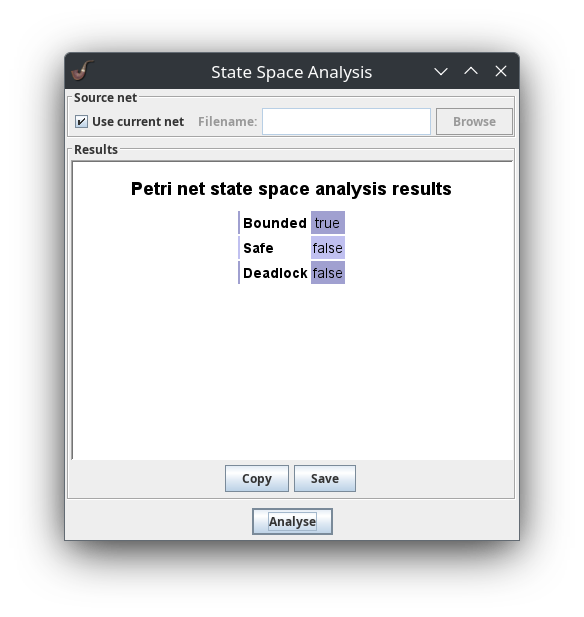
\includegraphics[width=7cm]{Screenshot_20240107_150221.png}\]

    \hypertarget{zadanie-5}{%
\subsection{Zadanie 5}\label{zadanie-5}}

Sieć reprezentująca problem producenta i konsumenta z nieograniczonym
buforem wygląda następująco:

\begin{figure}
\centering
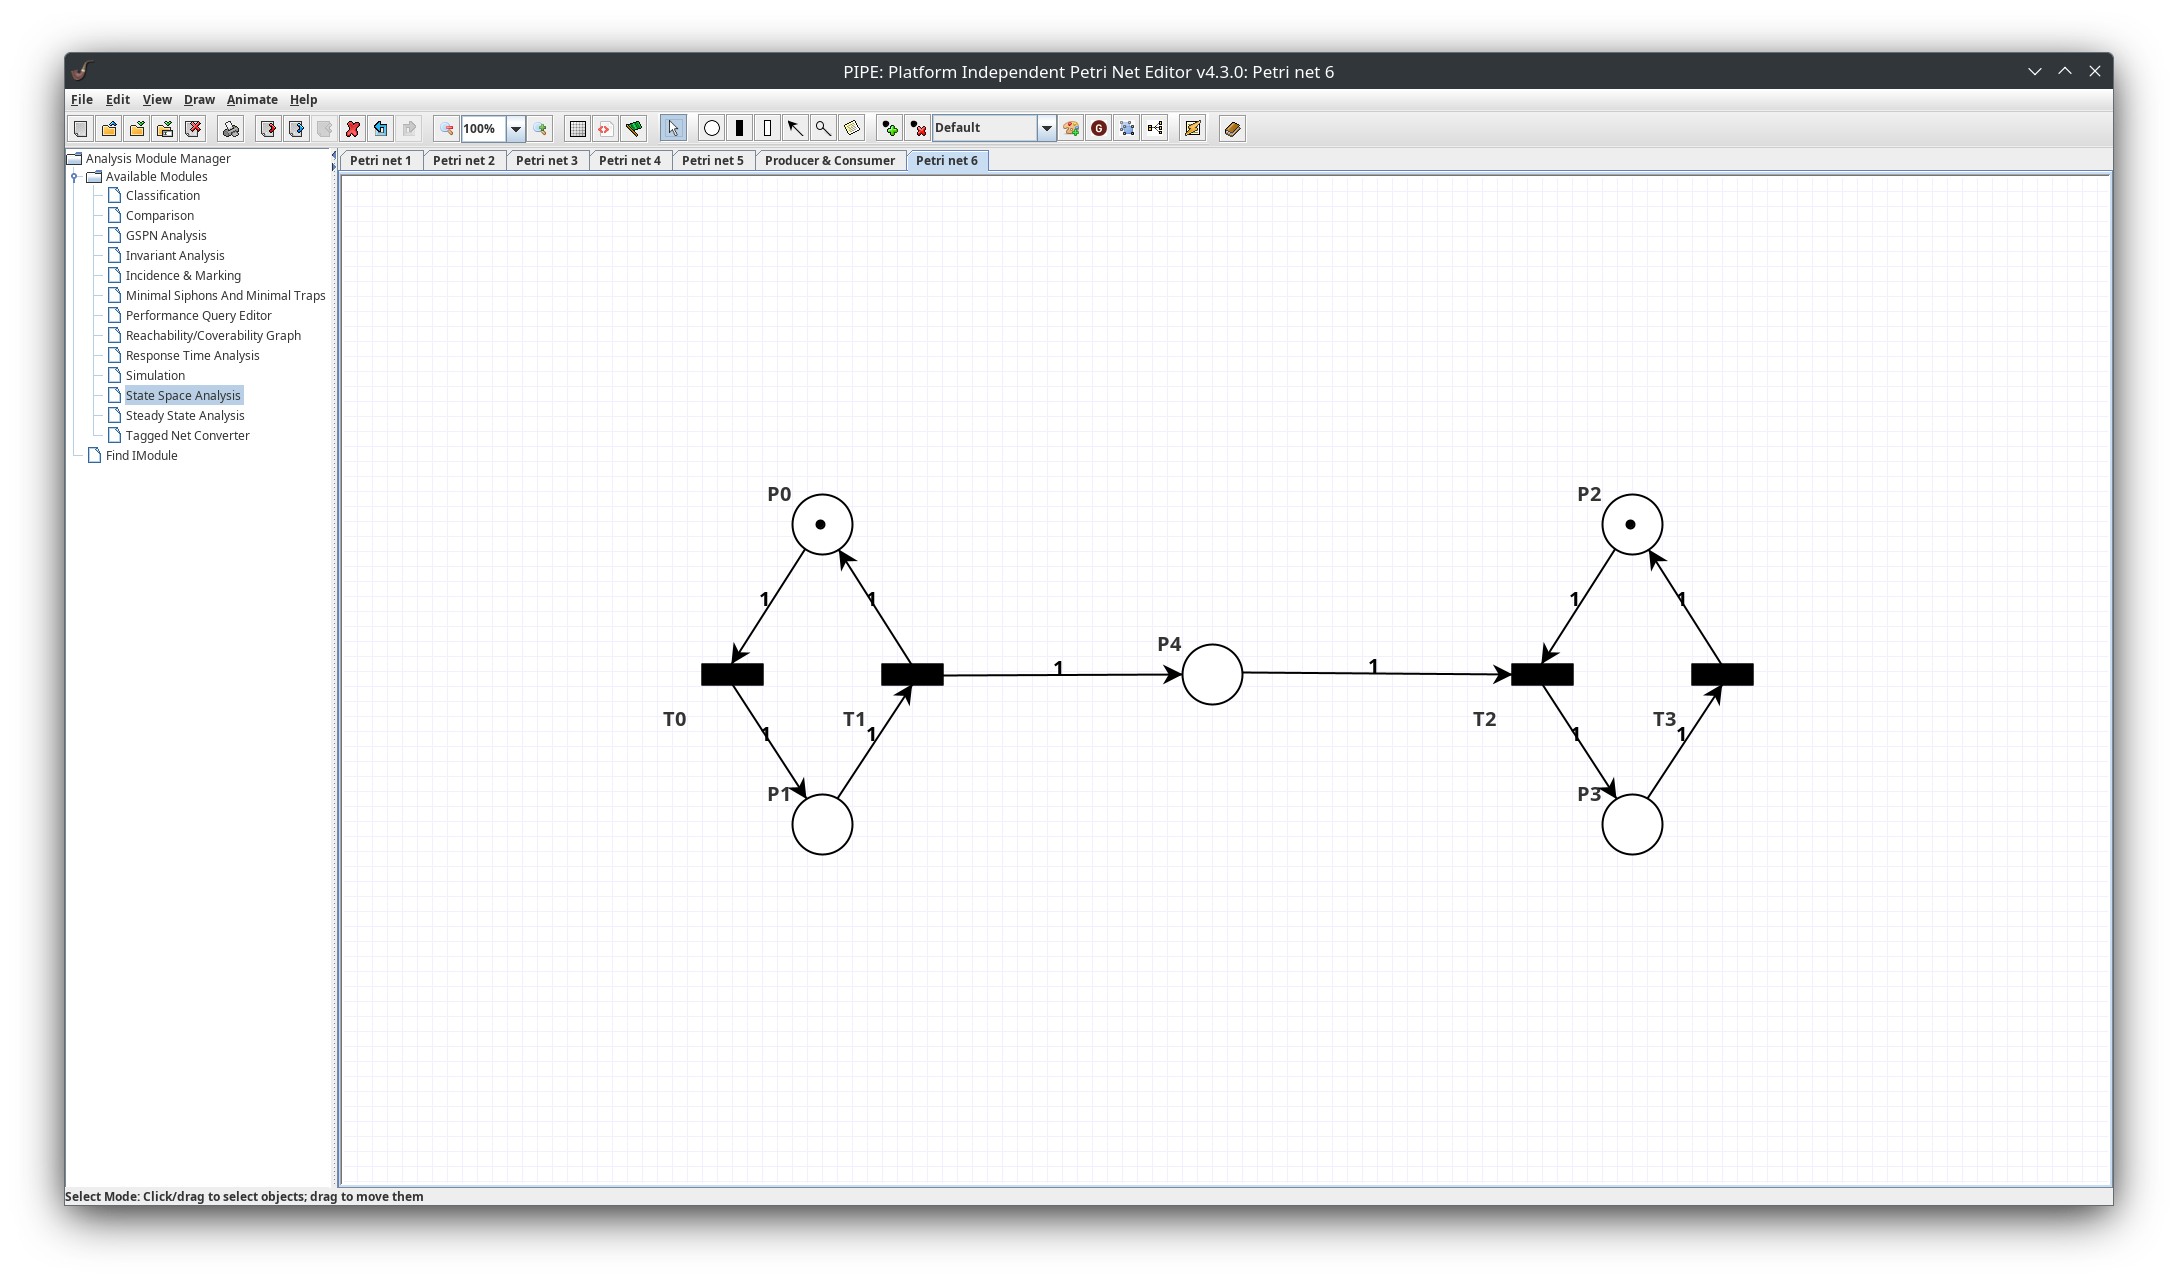
\includegraphics{Screenshot_20240107_151532.png}
\caption{Screenshot\_20240107\_151532.png}
\end{figure}

    \hypertarget{analiza-niezmiennikuxf3w}{%
\subsubsection{Analiza niezmienników}\label{analiza-niezmiennikuxf3w}}

Wynik dokonanej analizy niezmienników jest przedstawiony na obrazku
poniżej:

\[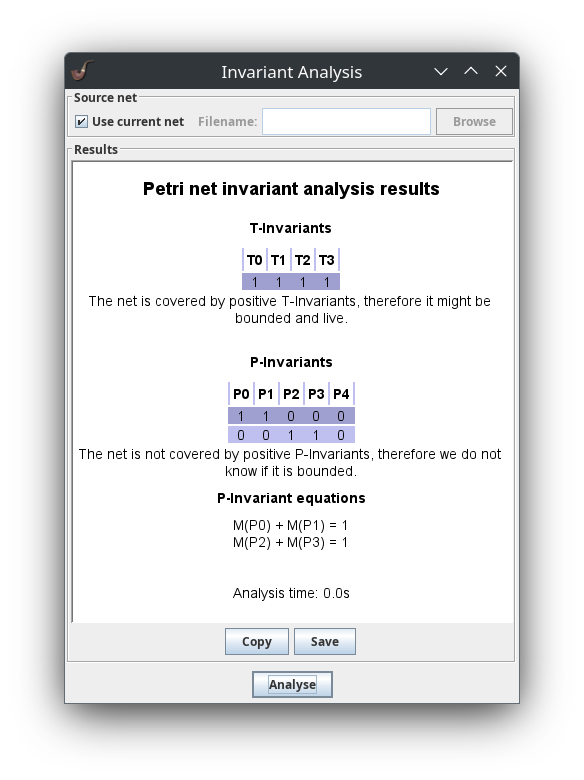
\includegraphics[width=7cm]{Screenshot_20240107_151707.png}\]

Obserwujemy brak pełnego pokrycia miejsc: miejsce \(P_4\) nie występuje
w żadnym równaniu.

    \hypertarget{analiza-stanuxf3w}{%
\subsubsection{Analiza stanów}\label{analiza-stanuxf3w}}

Jak wynika z \emph{State Space Analysis}, ta sieć:

\begin{itemize}
\tightlist
\item
  Nie jest ograniczona
\item
  Nie jest bezpieczna
\item
  Nie zawiera deadlocku
\end{itemize}

\[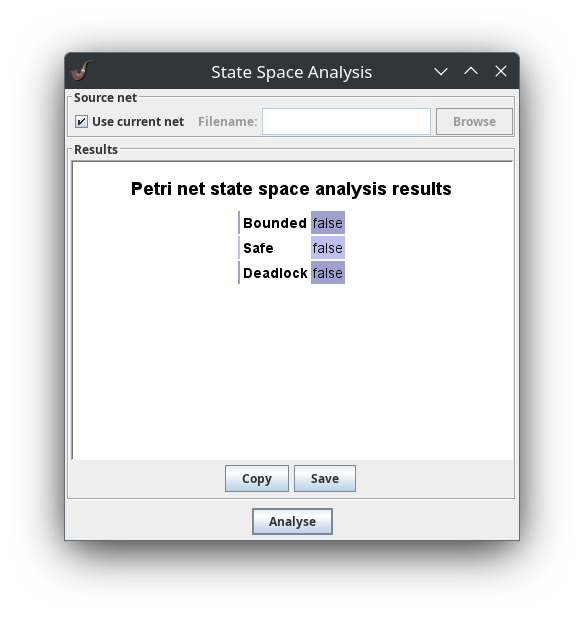
\includegraphics[width=7cm]{Screenshot_20240107_151833.png}\]

    \hypertarget{zadanie-6}{%
\subsection{Zadanie 6}\label{zadanie-6}}

Przykład sieci z możliwością zakleszczenia wygląda w sposób następujący:

\begin{figure}
\centering
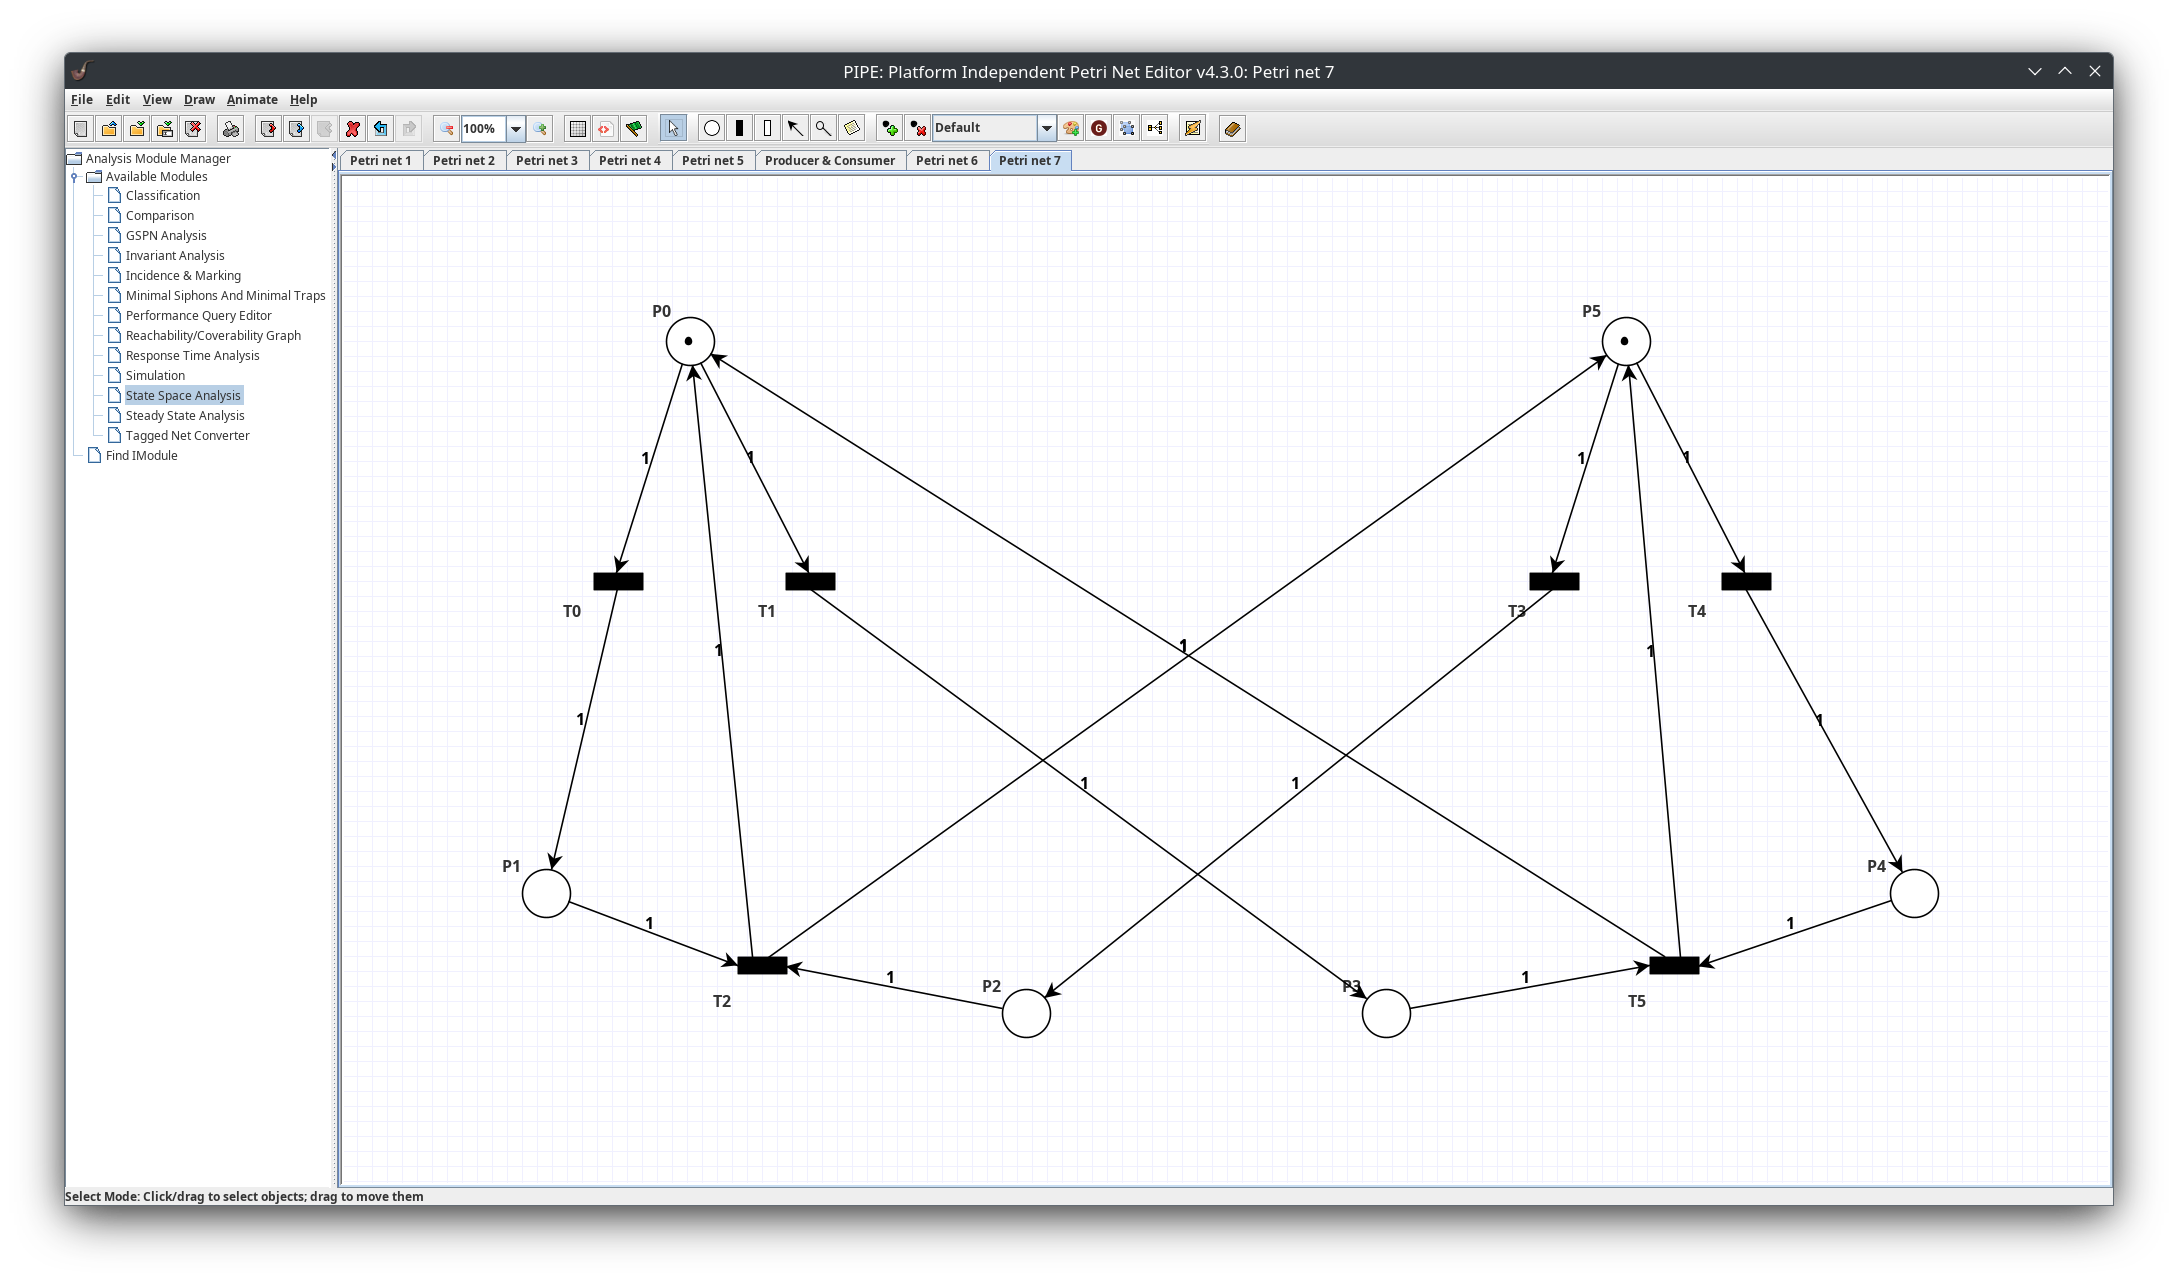
\includegraphics{Screenshot_20240107_153242.png}
\caption{Screenshot\_20240107\_153242.png}
\end{figure}

    \hypertarget{analiza-stanuxf3w}{%
\subsubsection{Analiza stanów}\label{analiza-stanuxf3w}}

Jak wynika z \emph{State Space Analysis}, ta sieć:

\begin{itemize}
\tightlist
\item
  Jest ograniczona
\item
  Jest bezpieczna
\item
  Zawiera deadlock (najkrótsza ścieżka prowadząca do deadlocku:
  \(T_0 T_4\))
\end{itemize}

\[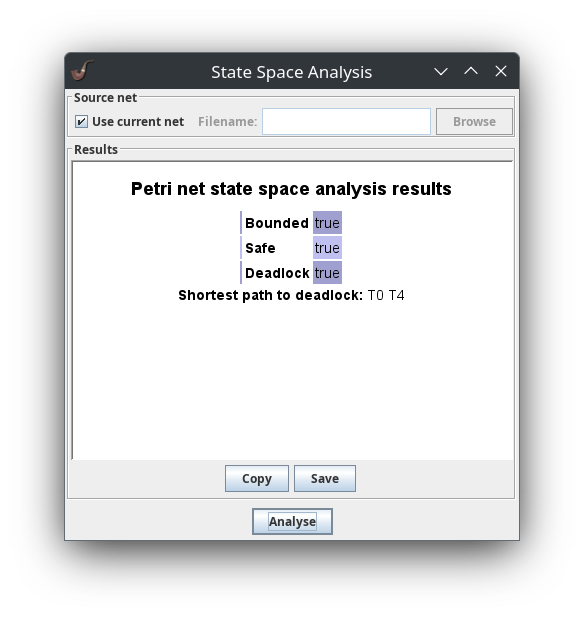
\includegraphics[width=7cm]{Screenshot_20240107_153314.png}\]

    \hypertarget{graf-osiux105galnoux15bci}{%
\subsubsection{Graf osiągalności}\label{graf-osiux105galnoux15bci}}

Został wygenerowany następujący graf osiągalności:

\[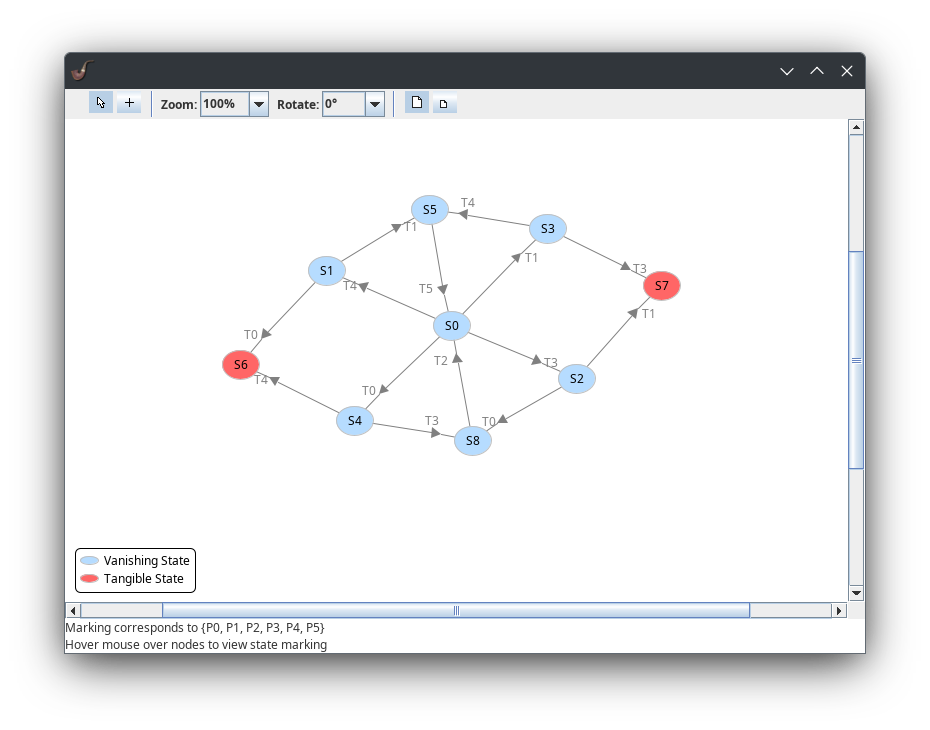
\includegraphics[width=7cm]{Screenshot_20240107_153547.png}\]

Jak widać, ze stanów \(S_6\) i \(S_7\) nie można wykonać żadnych przejść
(są zaznaczone na czerwono).

    \hypertarget{wnioski}{%
\section{Wnioski}\label{wnioski}}

\begin{itemize}
\item
  \textbf{Sieci Petriego} to graficzny język do modelowania i analizy
  systemów dyskretnych i współbieżnych, który używa miejsc, przejść i
  żetonów.
\item
  \textbf{Sieci Petriego mają różne własności}, takie jak ograniczoność,
  bezpieczeństwo, deadlock, zachowawczość, żywotność i odwracalność,
  które opisują ich zachowanie i możliwości.
\item
  \textbf{Graf osiągalności} to graf, który przedstawia wszystkie
  możliwe znakowania sieci Petriego i przejścia między nimi.
\item
  \textbf{Znaczniki} to elementy graficzne, które reprezentują dane,
  zasoby lub stany systemu. Znaczniki mogą być przemieszczane pomiędzy
  miejscami poprzez przejścia.
\item
  \textbf{Niezmienniki} to równania lub wektory, które opisują
  zachowanie sieci Petriego niezależnie od znakowania. Niezmienniki są
  używane do weryfikacji własności sieci Petriego, takich jak
  zachowawczość czy ograniczoność.
\item
  \textbf{Sieci Petriego mają wiele zastosowań} w różnych dziedzinach,
  takich jak automatyka, bioinformatyka, inżynieria oprogramowania,
  programowanie równoległe i inne.
\end{itemize}

    \hypertarget{bibliografia}{%
\section{Bibliografia}\label{bibliografia}}

\begin{enumerate}
\def\labelenumi{\arabic{enumi}.}
\item
  Materiały do laboratorium 12, dr inż. Włodzimierz Funika:\\
  \url{https://home.agh.edu.pl/~funika/tw/lab-petri/}
\item
  Sieci Petriego, dr inż. Jędrzej Ułasiewicz:\\
  \url{http://jedrzej.ulasiewicz.staff.iiar.pwr.wroc.pl/ProgramowanieWspolbiezne/wyklad/Sieci-Petriego15.pdf}
\item
  Platform Independent Petri net Editor 2 (PIPE2):\\
  \url{https://pipe2.sourceforge.net/}
\end{enumerate}


    % Add a bibliography block to the postdoc
    
    
    
\end{document}
